%!TEX root = ../thesis_a4.tex

\chapter{Melody Descriptors and Representations}
\label{chap:data_preprocessing}

\section{Introduction}
\label{sec:data_preprocessing_intro}

In this chapter, we describe methods for extracting relevant melodic descriptors and low-level melody representation from raw audio signals.  These melodic features are used as inputs to perform higher level melodic analysis by the methods described in the subsequent chapters. Since these features are used in a number of computational tasks, we consolidate and present these common processing blocks in the current chapter. This chapter is largely based on our published work presented in~\cite{Gulati2014Tonic,gulati2014Landmark,gulati_SITIS_2014}.

There are four sections in this chapter, and in each section, we describe the extraction of a different melodic descriptor or a representation.
\begin{itemize}
	\item In \secref{sec:data_preprocessing_tonic_identification}, we focus on the task of automatically identifying the tonic pitch in an audio recording. Our main objective is to perform a comparative evaluation of different existing methods and select the best method to be used in our work.
	\item In \secref{sec:data_preprocessing_melody_processing}, we present the method used to extract the predominant pitch from audio signals, and describe the post-processing steps to reduce frequently occurring errors.
	\item In \secref{sec:pre_processing_nyas_segmentation}, we describe our \gls{nyas}-based approach for segmenting melodies in Hindustani music. 
	\item In \secref{sec:pre_processing_tani_segmentation}, we describe the process of segmenting the solo percussion regions (\Gls{tani} sections) in the audio recordings of Carnatic music.  
\end{itemize}
	
%Along with the description of these method we also provide relevant implementation details and their default parameter settings. 

\section{Tonic Identification: Approaches and Comparative Evaluation}
\label{sec:data_preprocessing_tonic_identification}

The tonic pitch of a lead artist in \gls{iam} is the base frequency that serves as a reference and foundation for melodic integration throughout the performance. All the tones in the musical progression are always in reference and related to the tonic pitch (\secref{sec:melody_in_iam}). Therefore, for a meaningful comparison of melodies across recordings, it is important that the melodic representation is normalized by the tonic pitch in the recording. Identification of the tonic pitch in an audio recording thus becomes a crucial first step in melodic analysis of \gls{iam}. 

There exist a number of approaches for identifying tonic pitch in an audio recording of \gls{iam}~\citep{salamon2012multipitch,gulati2012two,bellur2012knowledge,ranjani2011carnatic,Sengupta2005b,chordia2013joint}. We present a detailed review of these approaches in \secref{sec:background_relevant_work_tonic_identification}. In our previous studies on tonic identification we showed promising results with identification accuracies close to 90\%~\citep{salamon2012multipitch,gulati2012two}. Similar accuracies are reported in other studies~\citep{ranjani2011carnatic,bellur2012knowledge}. As seen in our review (\secref{sec:background_relevant_work_tonic_identification}), it is misleading to draw a consensus on the best performing method just based on the accuracy reported in the publications. It is because these approaches are evaluated using different datasets with varied musical characteristics and under different experimental setup. 

In order to identify the most reliable, robust, and scalable approach, we perform their comparative evaluation using the same music collection and the same experimental setup. For this, we use a number of sizable datasets with varied musical and acoustical characteristics that are representative of the audio collections in \gls{iam}. In the subsequent sections, we describe the comparative evaluation, which is based on our earlier work presented in~\cite{Gulati2014Tonic}. The experimental setup and the datasets used for the evaluation are described in~\secref{sec:pre_processing_experimental_setup}. A detailed discussion of the results of the evaluation along with an in depth error analysis is presented in~\secref{sec:pre_processing_tonic_identification_results}. We then explain a heuristic-based majority voting process to correct the frequently occurring errors in tonic identification~(\secref{sec:pre_processing_tonic_identification_correcting_errors}). 


\subsection{Comparative Evaluation Setup}
\label{sec:pre_processing_experimental_setup}

We evaluate seven of the nine tonic identification methods listed in \tabref{tab:pre_processing_tonic_identification_summary_methods}. The methods selected for evaluation are
denoted by \acrshort{tonicid_justin}~\citep{salamon2012multipitch}, \acrshort{tonicid_sankalp}~\citep{gulati2012two}, \acrshort{tonicid_ranjani_1} and \acrshort{tonicid_ranjani_2}~\citep{ranjani2011carnatic}, \acrshort{tonicid_ashwin_1}, \acrshort{tonicid_ashwin_2} and \acrshort{tonicid_ashwin_3}~\citep{bellur2012knowledge}. Note that \acrshort{tonicid_sengupta}~\citep{Sengupta2005b} was not available for
evaluation and \acrshort{tonicid_chordia}~\citep{chordia2013joint} was not available when the experiments were conducted. 

Each of the method mentioned above is evaluated using six different datasets, \acrshort{tds_cm1}, \acrshort{tds_cm2}, \acrshort{tds_cm3}, \acrshort{tds_iitm1}, \acrshort{tds_iitm2} and \acrshort{tds_iisc}. A detailed description of these datasets in terms the musical material and the audio quality is given in~\secref{sec:corpus_tonic_datasets}. A summary of the datasets can be obtained from~\tabref{tab:tonic_datasets}. The diversities present in \gls{iam} repertoire in terms of the musical and acoustical characteristics are well captured in these six datasets. Note that \acrshort{tonicid_ashwin_1} method requires several excerpts from the same concert as an input, which is only available in the case of \acrshort{tds_iitm1} dataset. Hence, \acrshort{tonicid_ashwin_1} is only evaluated using \acrshort{tds_iitm1} dataset.

For vocal performances, we evaluate the accuracy of correctly identifying the tonic pitch, whereas, for instrumental music, we evaluate the accuracy of identifying the tonic pitch-class only (i.e.~the identified tonic pitch is allowed to be in any octave). This is because whilst for vocal music the concept of the tonic pitch being in a specific octave is clearly defined (because it is restricted by the pitch range of the singer), this notion is not as clear for instrumental music. For vocal performances, the tonic identified by a method is considered as correct if it lies within 50\,Cents of the ground truth annotation. For instrumental music, output of a method is considered as correct if it is within 50\,Cents of the correct tonic pitch-class.

Classification-based methods (\acrshort{tonicid_justin} and \acrshort{tonicid_sankalp}) are evaluated by using 10-fold cross-validation methodology on every dataset. The experiments are repeated 10 times and the mean accuracy over the 10 repetitions are reported. Parameters for all the methods are kept fixed across all datasets. Since the tonic pitch range for male and female singers, and for instrumental music is different, editorial metadata regarding the gender of the singer and the type of music excerpt (vocal or instrumental) can be used to improve the accuracy of tonic identification. We therefore perform two sets of experiments, first one, using only the audio excerpts, and the other, in which the methods are also given information about the gender of the singer and the type of excerpt (vocal or instrumental). The results of these evaluations are presented in the subsequent section. We remind again that a brief description of the methods considered in this evaluation is provided in \secref{sec:background_relevant_work_tonic_identification}.


\subsection{Results and Discussion}
\label{sec:pre_processing_tonic_identification_results}

In this section, we present the results of the comparative evaluation. We compare the performance of different tonic identification approaches, highlight their shortcomings and discuss various types of errors made by them. The section is divided into three parts. In ~\secref{sec:pre_processing_tonic_id_results_only_audio_data}, we present the results obtained when only the audio data is used and no additional metadata is provided to the methods. Subsequently, we report the performance accuracy
obtained when information regarding the gender of the singer (male or female) and performance type (instrumental or vocal) is also provided to the methods in addition to the audio data (\secref{sec:pre_processing_tonic_id_results_with_metadata}). Finally, in \secref{sec:pre_processing_tonic_identification_error_analysis}, we present an analysis of the most common mistakes made by the methods and make some general observations regarding their performances.


\subsubsection{Results Obtained Using Only Audio Data}
\label{sec:pre_processing_tonic_id_results_only_audio_data}

In Table~\ref{tab:tonic_identification_accuracy_without_gender_info}, we summarize the
identification accuracies (in percentage) for tonic pitch (TP) and tonic
pitch-class (TPC) obtained by seven methods on six datasets, using
only audio data.

{\renewcommand{\arraystretch}{1.4}
\setlength{\tabcolsep}{10pt}
\begin{sidewaystable}
	\centering
	\begin{tabular}{ c | c  c : c  c : c  c : c  c : c  c : c  c }
\tabletop
		\multirow{2}{*}{Methods}  & \multicolumn{2}{ c: }{\acrshort{tds_cm1}} & \multicolumn{2}{ c: }{\acrshort{tds_cm2}} & \multicolumn{2}{ c: }{\acrshort{tds_cm3}}  &    \multicolumn{2}{ c: }{\acrshort{tds_iisc}}  &  \multicolumn{2}{ c: }{\acrshort{tds_iitm1}}  & \multicolumn{2}{ c}{\acrshort{tds_iitm2}} \\
		\cline{2-13}
		{} & TP & TPC    & TP & TPC & TP & TPC & TP & TPC
		& TP & TPC & TP & TPC   \\
\tablemid
		\acrshort{tonicid_justin} & - & 88.9 & 87.4 & 90.1 & \textbf{88.4} & \textbf{91} & 75.6 & 77.5 & 	89.5 & \textbf{97.4} & 90.8 & \textbf{94.1}\\

		\acrshort{tonicid_sankalp} & - & \textbf{92.2} & \textbf{87.8} & \textbf{90.9} & 87.7 & 90.5 &
		79.8 & \textbf{85.3} & \textbf{97.4} & \textbf{97.4} & \textbf{93.6}
		& 93.6  \\
		
		\hdashline
		
		\acrshort{tonicid_ranjani_1} & - & 81.4 & 69.6 & 84.9 & 73.2 & 90.8 & 81.8 & 83.6 & 92.1 & \textbf{97.4} &
		80.2 & 86.9  \\
		
		\acrshort{tonicid_ranjani_2} & - & 63.2 & 65.7 & 78.2 & 68.5 & 83.5 & \textbf{83.6} & 83.6 & 94.7 &
		\textbf{97.4} & 83.8 & 88.8\\
		
		\acrshort{tonicid_ashwin_1} & - & - & - & - & - & - & - & - & 89.5 & 89.5 & - & - \\
		
		\acrshort{tonicid_ashwin_2} & - & 88.9 & 74.5 & 82.9 & 78.5 & 83.4 & 72.7 & 76.4 & 92.1 & 92.1 & 86.6   & 89.1 \\
		
		\acrshort{tonicid_ashwin_3} & - & 86 & 61.1 & 80.5 & 67.8 & 79.9 & 72.7 & 72.7 & 94.7 & 94.7 & 85  & 86.6 \\
\tablebot
	\end{tabular}
	\caption[Tonic identification accuracies of seven methods on six different datasets using only audio data]{Accuracies for tonic pitch (TP \%) and tonic pitch-class (TPC \%) identification by seven methods on six different datasets using only audio data. The best accuracy obtained for each dataset is
	highlighted using bold text. The dashed horizontal line divides the methods based on supervised learning (\acrshort{tonicid_justin} and \acrshort{tonicid_sankalp}) and those based on expert knowledge (\acrshort{tonicid_ranjani_1}, \acrshort{tonicid_ranjani_2}, \acrshort{tonicid_ashwin_1}, \acrshort{tonicid_ashwin_2} and \acrshort{tonicid_ashwin_3}). TP column for \acrshort{tds_cm1} is marked as `-', because it consists of only instrumental excerpts for which we not evaluate tonic pitch accuracy. \acrshort{tonicid_ashwin_1} is only evaluated on \acrshort{tds_iitm1} since it works on the whole concert recording.}
	\label{tab:tonic_identification_accuracy_without_gender_info}
\end{sidewaystable}

From \tabref{tab:tonic_identification_accuracy_without_gender_info}, we see that most of the methods perform well on all the datasets, and the accuracy of the best performing method on each dataset ranges from 84-97\%. We note that the identification accuracy obtained for instrumental music (\acrshort{tds_cm1}) by each method is comparable to the accuracy obtained for vocal music, meaning the approaches are equally suitable for vocal and instrumental music. The approaches based on multipitch analysis and classification (\acrshort{tonicid_justin} and \acrshort{tonicid_sankalp}) are more consistent and perform better across different datasets compared to the approaches based only on the predominant pitch (with the exception of \acrshort{tds_iisc}, which is due its poor recording quality). We see that the performance of the two multipitch-based approaches is comparable. As could be expected, a simple maximum peak selection approach employed by \acrshort{tonicid_ashwin_1} and \acrshort{tonicid_ashwin_3} is too simplistic and the template matching approach employed in \acrshort{tonicid_ashwin_2} yields better results in most cases. 

\acrshort{tonicid_sankalp} obtains the best results for the instrumental dataset \acrshort{tds_cm1}, with \acrshort{tonicid_ashwin_2} and \acrshort{tonicid_justin} reporting comparable accuracies. For the \acrshort{tds_cm2} and \acrshort{tds_cm3} datasets, we see that the multipitch-based approaches (\acrshort{tonicid_justin} and \acrshort{tonicid_sankalp}) obtain the best performance, whilst the predominant pitch-based methods exhibit a considerable difference between the TP and TPC accuracies. This means that in many cases these approaches are able to identify the tonic pitch-class correctly but fail to identify the correct octave of the tonic pitch. In the case of \acrshort{tonicid_ranjani_1}, \acrshort{tonicid_ranjani_2}, \acrshort{tonicid_ashwin_2} and \acrshort{tonicid_ashwin_3}, this can be attributed primarily to the tonic selection procedure employed by these approaches. The group-delay processing used in \acrshort{tonicid_ashwin_2} and \acrshort{tonicid_ashwin_3}, and the estimators used in \acrshort{tonicid_ranjani_1} and \acrshort{tonicid_ranjani_2}, accentuate the peaks corresponding to all \glspl{svara} that have a low degree of pitch variance. This includes both the lower and higher octave \gls{shadja} and \gls{panchama} in addition to the middle octave \gls{shadja} (the tonic pitch). Furthermore, the magnitude of peaks corresponding to \gls{shadja} in higher and lower octave is sometimes further accentuated by pitch halving and doubling errors produced by the pitch extraction algorithm. This makes identification of the correct tonic octave more difficult, and as seen in Table~\ref{tab:tonic_identification_accuracy_without_gender_info}, it results in a higher degree of octave errors.

When considering the results for the \acrshort{tds_iisc} dataset, we note that the performance drops for all methods. The main reason for this is the poor audio quality of the excerpts in this collection. The recordings are relatively old and noisy, and contain a humming sound in the background. This makes pitch
tracking very difficult. Furthermore, the drone sound in the recordings is very weak compared to the lead artist, which explains the drop in performance for the multipitch-based approaches. On the other hand, if we consider performance for \acrshort{tds_iitm1}, we see that all methods perform very well. This is because each excerpt in this dataset is a full concert, which includes many performances in different \glspl{raga}. Usually different set of \glspl{svara} are used in different performances, but with the same tonic pitch throughout the concert. As a result, the pitch histogram contains a high peak corresponding to the Sa \gls{svara}, which makes the identification of the tonic pitch easier.

\begin{figure}
	\begin{center}
		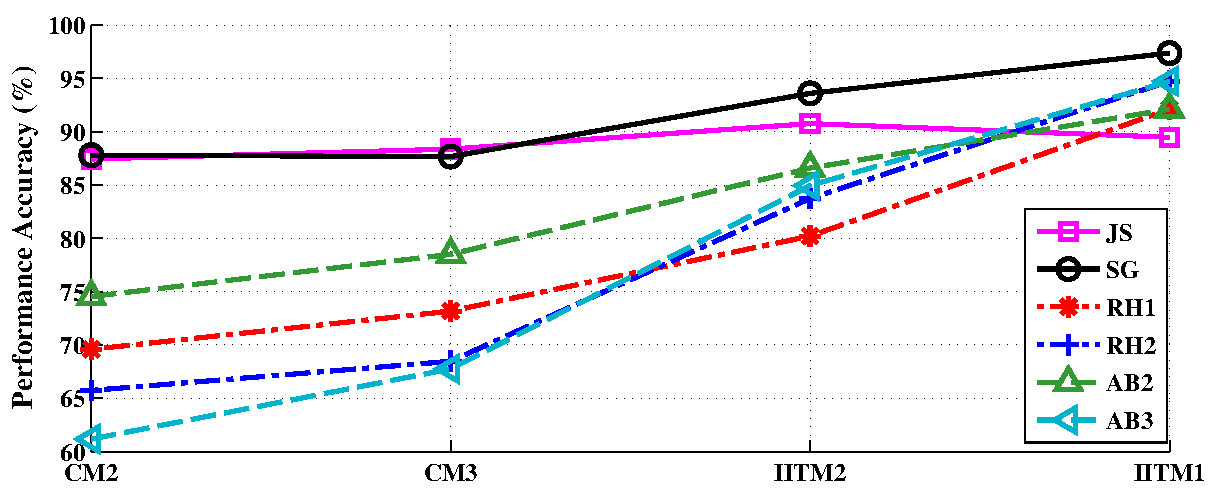
\includegraphics[width=\figSizeNinety]{ch05_preprocessing/figures/Accuracy_Length.pdf}
	\end{center}
	\caption[Tonic identification accuracies of different approaches on four datasets]{Accuracy (\%) of different methods on four datasets arranged by increasing order of mean duration. Only the subscript in the names of the methods and datasets is used for labeling the axis and legends.}
	\label{fig:tonic_id_accuracy_vs_length}
\end{figure}


We now proceed to analyze the tonic identification accuracy as a function of the excerpt duration. As shown in~\tabref{tab:tonic_datasets}, different datasets contain audio excerpts of different lengths. In order to investigate a possible correlation between the accuracy of a method and the length of an audio
excerpt, in~\figref{fig:tonic_id_accuracy_vs_length}, we plot the identification accuracies of different methods for four of the six datasets ordered
by the mean duration of the excerpts: \acrshort{tds_cm2} (3 min), \acrshort{tds_cm3} (full song), \acrshort{tds_iitm2} (full song) and \acrshort{tds_iitm1} (full concert). \acrshort{tds_cm1} and \acrshort{tds_iisc} are excluded because the characteristics of these datasets are very different compared to the rest of the datasets (\acrshort{tds_cm1} contains only instrumental performances and \acrshort{tds_iisc} has poor quality audio). As could be expected, from~\figref{fig:tonic_id_accuracy_vs_length} we notice that practically for all methods there is an improvement in the performance as we increase the duration
of the excerpts. Interestingly, the improvement is very significant for the predominant pitch-based methods (\acrshort{tonicid_ranjani_1}, \acrshort{tonicid_ranjani_2}, \acrshort{tonicid_ashwin_2} and \acrshort{tonicid_ashwin_3}) compared to the multipitch-based methods (\acrshort{tonicid_justin} and \acrshort{tonicid_sankalp}). This shows that the latter approaches, which exploit the pitch information of the drone instrument require less amount of audio data to perform this task. Notably, the accuracy of \acrshort{tonicid_justin} remains nearly the same across all the datasets, which is because the normalized distribution of the tones corresponding to the drone sound remains the same throughout the excerpt. Since this method does not utilize the predominant pitch information, it does not benefit much from the long duration audio excerpts. Note that, while the TP accuracy by \acrshort{tonicid_justin} is the lowest compared to the other methods on \acrshort{tds_iitm1} dataset, the TPC accuracy is amongst the highest. 

\begin{figure}
	\begin{center}
		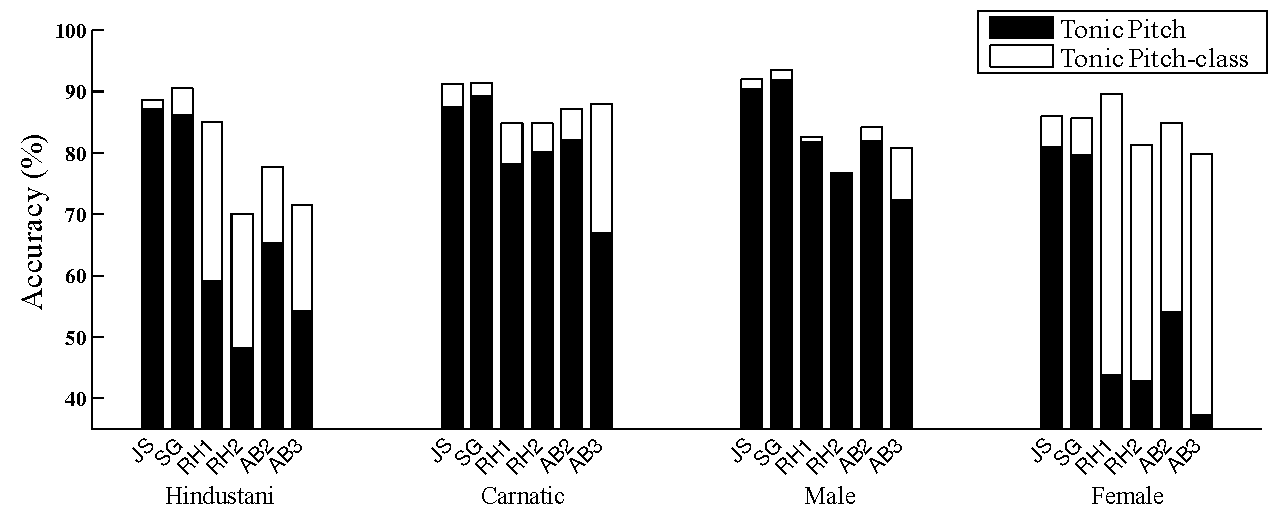
\includegraphics[width=\figSizeHundred]{ch05_preprocessing/figures/Category_Performance.pdf}
	\end{center}
	\caption[Tonic identification accuracies for Hindustani, Carnatic, male and female excerpts]{Accuracy (\%) as a function of different attributes (Hindustani, Carnatic, male, female).Only the subscript in the names of the methods is used for labeling the axis.}
	\label{fig:tonic_id_categorywise_performance}
\end{figure}

In addition to analyzing the performance accuracy for the whole dataset, we also examine the results as a function of different musical attributes of a dataset, namely music tradition (Hindustani or Carnatic) and the gender of the lead singer (male or female). For this analysis, we use the \acrshort{tds_cm2} dataset, as it has the most balanced representation of excerpts from the different categories. In~\figref{fig:tonic_id_categorywise_performance}, we show the accuracies obtained by the different methods as a function of the different attributes. We see that the performance of the multipitch-based approaches (\acrshort{tonicid_justin} and \acrshort{tonicid_sankalp}) is relatively independent of the music tradition (Hindustani or Carnatic). On the other hand, for the predominant pitch-based approaches there is a significant difference in performance for Hindustani and Carnatic music. They obtain considerably better results on Carnatic music. The most notable difference for these approaches is the increased amount of octave errors made for Hindustani music compared to Carnatic music (deduced from the difference seen in tonic pitch-class and the tonic pitch accuracies). A possible reason for this is that in the Hindustani recordings the \gls{tanpura} is generally more salient compared to the Carnatic recordings. This results in the monophonic pitch estimators tracking the \gls{tanpura} in some frames, in particular, when the lead artist is not singing. As a result, the pitch histogram includes high peaks at octave multiples or sub-multiples of the correct tonic pitch. In the case of \acrshort{tonicid_ashwin_2}, \acrshort{tonicid_ashwin_3}, \acrshort{tonicid_ranjani_1} and \acrshort{tonicid_ranjani_2}, most octave errors were found to be sub-multiples of the tonic pitch, possibly caused by the salient lower Sa played by the drone instrument.

Now we turn to examine the performance as a function of the gender of the lead artist (male or female). We see that in general, all the approaches function better
for the performances by the male singers compared to those by the female singers. Similar to the case across music traditions, the difference is more significant for the predominant pitch-based methods, which make a large number of octave errors for the performances by the female singers. As noted earlier (\secref{sec:tonic_selection}), in methods \acrshort{tonicid_ranjani_1}, \acrshort{tonicid_ranjani_2}, \acrshort{tonicid_ashwin_2} and \acrshort{tonicid_ashwin_3} a range of 100-250 Hz is considered for finding the tonic pitch when no additional metadata about the artists is available. In the case of female singers, the tonic usually resides in the higher end of this range. However, the presence of the drone, the tonal sounds produced by percussive instruments and the octave errors produced by the pitch tracker, all contribute to the appearance of a high peak one octave below the tonic of the female singers. This is especially the case for three minute excerpts, wherein a limited amount of vocal pitch information is available. In the case of the approaches based on multipitch analysis and classification (\acrshort{tonicid_justin} and \acrshort{tonicid_sankalp}), a probable reason for obtaining better performance for male singers is the larger number of excerpts from male singers in the database. As a result, it is possible that the rules learned by the classifier are slightly biased towards the performances of male singers.


\subsubsection{Results Obtained Using Metadata Together with the Audio}
\label{sec:pre_processing_tonic_id_results_with_metadata}

One of the ways to reduce the amount of octave errors in tonic identification is to restrict the frequency range of the allowed tonic pitches. The frequency range can be optimized based on the additional information regarding the gender of the singer (when available) to guide the method. In this section, we analyze the effect of including information regarding the gender of the singer and the performance type (vocal or instrumental) on the identification accuracy obtained by the methods.

\setlength{\tabcolsep}{4pt}
\begin{table}
\begin{centering}
	\begin{tabular}{ c | c  c  c  c  c  c }
\tabletop
		{Methods}  & \acrshort{tds_cm1} & \acrshort{tds_cm2} & \acrshort{tds_cm3} &	\acrshort{tds_iisc} & \acrshort{tds_iitm1} & \acrshort{tds_iitm2}\\
\tablemid
		\acrshort{tonicid_justin} & 88.9 & \textbf{93.6} & 92.4 & 80.9 & \textbf{97.4} & 92.3 \\
		
		\acrshort{tonicid_sankalp} & 92.2 & 90.9 & 90.5 & 85.3 & \textbf{97.4} & \textbf{93.6}  \\
		\hdashline
		\acrshort{tonicid_ranjani_1} & 87.7 & 83.5 & 88.9 & \textbf{87.3} &\textbf{ 97.4} & 91.7 \\
		
		\acrshort{tonicid_ranjani_2} & 79.55 & 76.3 & 82 & 85.5 & \textbf{97.4} & 91.5 \\
		
		\acrshort{tonicid_ashwin_1} & - & - &- & - & \textbf{97.4} & - \\
		
		\acrshort{tonicid_ashwin_2} & \textbf{92.3} & 91.5 & \textbf{94.2} & 81.8 & \textbf{97.4} & 91.1 \\
		
		\acrshort{tonicid_ashwin_3} & 87.5 & 86.7 & 90.9 & 81.8 & \textbf{94.7} & 89.9 \\
\tablebot		
	\end{tabular}
\par	\end{centering}
	\caption[Tonic identification accuracies of seven methods on six different datasets using both audio and editorial metadata]{Accuracies (tonic pitch-class (\%)) when additional information regarding the gender of the lead singer (male/female) and performance type (vocal/instrumental) is used. The dashed horizontal line divides the methods based on supervised learning (\acrshort{tonicid_justin} and \acrshort{tonicid_sankalp}) and those based on expert knowledge (\acrshort{tonicid_ranjani_1}, \acrshort{tonicid_ranjani_2}, \acrshort{tonicid_ashwin_1}, \acrshort{tonicid_ashwin_2} and \acrshort{tonicid_ashwin_3}).}
	\label{tab:tonic_identification_accuracy_with_gender_info}
\end{table}

In~\tabref{tab:tonic_identification_accuracy_with_gender_info}, we present the identification accuracies obtained when associated metadata is available to the methods in addition to the audio data. Note for this evaluation we only report the tonic pitch
accuracy for vocal excerpts (and not pitch-class accuracy) since when this metadata is available the pitch range of the tonic is known and limited to a
single octave, meaning the TP and TPC accuracies will be the same.

Comparing the identification accuracies summarized in~\tabref{tab:tonic_identification_accuracy_with_gender_info} with the with ones in~\tabref{tab:tonic_identification_accuracy_without_gender_info}, we see that the accuracies for all methods are higher when gender and performance metadata is available. With the additional information the performance of the predominant pitch-based approaches (\acrshort{tonicid_ashwin_2}, \acrshort{tonicid_ashwin_3} and \acrshort{tonicid_ranjani_1}) becomes closer to that of the multipitch-based approaches (\acrshort{tonicid_justin} and \acrshort{tonicid_sankalp}). Whilst the performance of all methods is improved, the increase in accuracy is more considerable for the predominant pitch-based approaches which use template matching (in particular \acrshort{tonicid_ashwin_2} and \acrshort{tonicid_ashwin_3}) compared to classification-based approaches (\acrshort{tonicid_justin} and \acrshort{tonicid_sankalp}). This possibly indicate that the rules learned automatically using machine learning are more complete compared to the relatively simple Sa-Pa templates, meaning that the classification-based approaches can correctly identify the octave of the tonic even without using gender metadata. That is, since both male and female excerpts are used during training, the influence of the gender of the singer on the pitch features is implicitly learned by the classifier, thus producing rules that can handle both male and female performances, even without explicit metadata about the gender of the singer. On the other hand, manually defined template-based approaches require this extra information to fine-tune the frequency range
considered for the tonic, after which they obtain comparable performance to that of the classification-based methods.

A potential advantage of the template-based approaches is that they do not require training. This, in theory, could make them more generalizable compared
to the classification-based methods. To assess this, we ran an experiment in which the classification-based approaches were trained on one dataset and tested on a different dataset (\acrshort{tds_cm2} and \acrshort{tds_iitm2}). We found that the results only went down by approximately 2\% compared to the results obtained using 10-fold cross validation on a single dataset. Furthermore, the datasets used for this experiment contained relatively different music material (percentage of Carnatic music excerpts and length of the audio files). This suggests that for tonic identification the rules learned by the classification-based approaches are generalizable and can be used to obtain high identification accuracies on diverse and sizable music collections of \gls{iam}.


\subsubsection{Error Analysis}
\label{sec:pre_processing_tonic_identification_error_analysis}

We now turn to analyze the different types of errors made by the methods, both with and without using additional metadata for each dataset. Overall, three common types of errors are identified: Pa errors, where the fifth (Pa) is selected instead of the tonic, Ma errors, where the fourth (Ma) is selected instead of the tonic, and the previously mentioned octave errors, where the correct pitch is identified but in the wrong octave (usually one octave above or below the
tonic). Since the octave errors are already discussed at length in the previous paragraphs, here we focus on all other types of errors, which we divide into three categories: Pa (for Pa errors), Ma (for Ma errors) and ``Other'', which includes all errors that are neither Pa, Ma nor octave errors (e.g.~selecting the seventh (\gls{ni}) instead of the tonic Sa).


\begin{figure}
	\begin{center}
		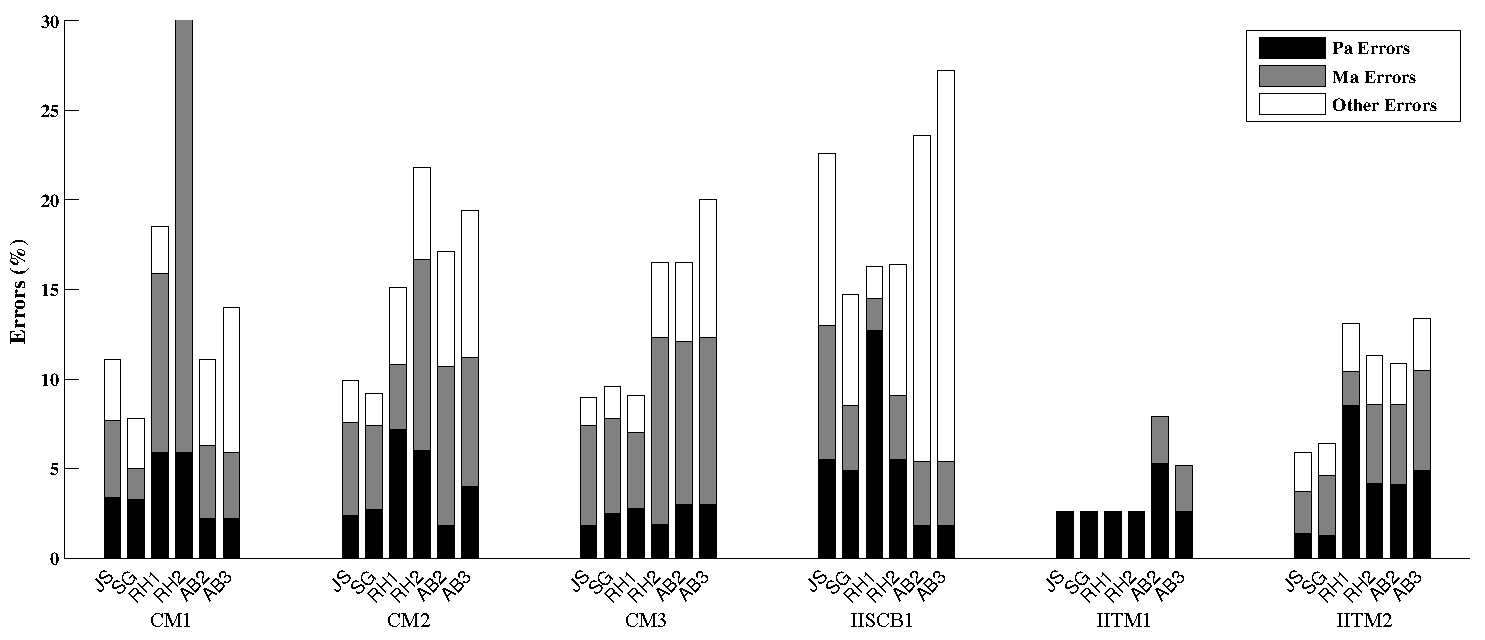
\includegraphics[width=\figSizeHundred]{ch05_preprocessing/figures/ErrorAnalysis_Without_MF.pdf}
	\end{center}
	\caption[Percentage of Pa, Ma and `Other' type errors in tonic identification]{The percentage of audio excerpts containing each of the three different categories of errors (excluding octave errors): Pa, Ma and Other, when no additional metadata is used. Only the subscript in the names of the methods and datasets is used for labeling the axis.}
	\label{fig:tonic_identification_errors_without_MF}
\end{figure}

In~\figref{fig:tonic_identification_errors_without_MF}, for each dataset, we show the percentage of excerpts containing each of the three categories of errors for every method (when no additional metadata is used). We see that for most datasets Pa and Ma errors constitute a large proportion of the total amount of errors made by each method. These confusions make sense from a musical perspective, since in every performance of \gls{iam} one of these two \glspl{svara} (Pa or Ma) is always present in a melody in addition to Sa (the tonic pitch-class). Furthermore, the pitch distance between Sa and Pa (fifth) is
the same as the distance between Ma and higher Sa, and the pitch distance between Sa and Ma (one fourth) is same as the distance between between Pa and higher Sa. Since most approaches are based on templates or rules that consider the pitch distance between the peaks of the feature histogram, these equivalences can
cause four types of confusions: considering a Sa-Pa pair to be Ma-Sa leading to a Pa error, considering Ma-Sa to be Sa-Pa leading to a Ma error, considering
Sa-Ma to be Pa-Sa leading to a Ma error and considering Pa-Sa to be Sa-Ma leading to a Pa error.

For the approaches based on multipitch analysis (\acrshort{tonicid_justin} and \acrshort{tonicid_sankalp}), we observe that the only case where we get more `Other' errors compared to Pa and Ma errors is for the \acrshort{tds_iisc} dataset. Since the drone sound is very weak in the excerpts of this dataset, there are cases in which the prominent peaks of the multipitch histogram correspond to \glspl{svara} other than Sa, Ma and Pa (which depends on the choice of the \gls{raga}). Since these approaches assume that the multipitch histogram represents the \glspl{svara} of the drone instrument, the peaks of the histogram are mistakenly identified as Sa and Pa or Sa and Ma, leading to an error in identification. For these specific type of excerpts the \acrshort{tonicid_ranjani_1} method produces slightly better results, as the \gls{shadja} is not inflected (i.e. there is little pitch variation within the \gls{svara}) regardless of the \gls{raga}.

\begin{figure}
	\begin{center}
		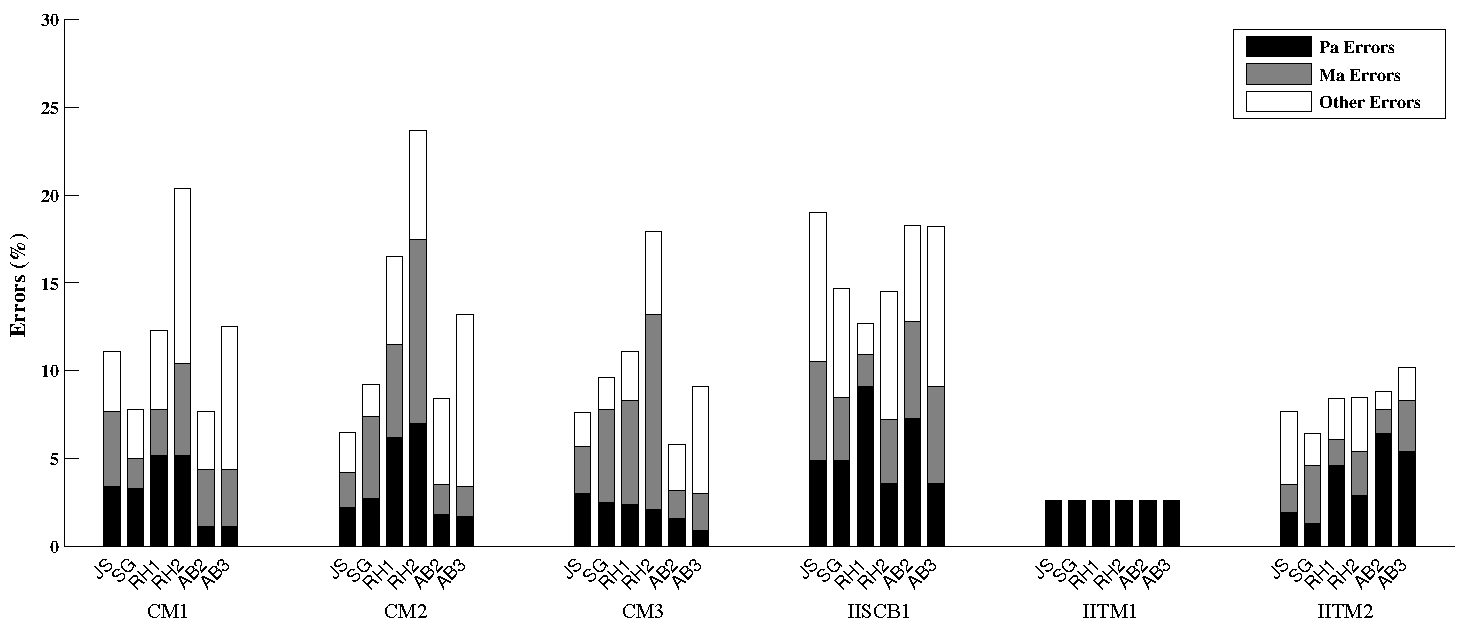
\includegraphics[width=\figSizeHundred]{ch05_preprocessing/figures/ErrorAnalysis_With_MF.pdf}
	\end{center}
	\caption[Percentage of Pa, Ma and `Other' type errors in tonic identification, using editorial metadata]{Percentage of different type of errors (Pa, Ma and Others) by different methods on all the datasets using information regarding the gender of the singer and performance type. Only the subscript in the names of the methods and datasets is used for labeling the axis.}
	\label{fig:tonic_identification_errors_with_MF}
\end{figure}

In many cases we observe that the percentage of Ma errors is greater than the percentage of Pa errors. For the classification-based approaches, this can be
attributed to the fact that in most excerpts the drone instrument is tuned to Pa tuning (lower Sa, middle Sa, middle Sa, lower Pa). This creates a
bias in the training set and the rules learned by the classifier work better for Pa tuning. Ma errors are also common in \acrshort{tonicid_ranjani_2}, as the estimator looks for a Sa-Pa-higher Sa pitch relation, which would also fit a Ma-tuned performance. \acrshort{tonicid_ranjani_1} on the other hand does not search for a Sa-Pa-Sa template, resulting in a low proportion of Ma errors compared to the other methods. Finally we note that most methods do not make any Ma errors on the \acrshort{tds_iitm1} dataset. This is because the items in this dataset are full concerts, each concert consisting of several pieces. Whilst Ma may be included in the melody of some of the pieces, Pa and Sa are always present. As a result, the pitch histogram for the complete concert does not contain a prominent Ma peak, meaning that it is highly unlikely for it to be selected as the tonic.



We examine how the errors are affected once we allow methods to use gender and performance metadata~(\figref{fig:tonic_identification_errors_with_MF}). If we compare the results to those in~\figref{fig:tonic_identification_errors_without_MF}, we see
that Ma and Pa errors are reduced more than ``Other'' errors. By restricting the tonic frequency range to a single octave we prevent the
appearance of a high Sa peak, thus avoiding the possible confusion between fourths and fifths explained earlier and reducing the amount of Pa and Ma errors.

For \acrshort{tonicid_ranjani_1} and \acrshort{tonicid_ranjani_2} the percentage of Ma errors actually increases slightly after including male/female information. A large proportion of these errors were observed in excerpts with female singers. For these excerpts, the range for \gls{shadja} candidates is limited to 130-250 Hz. For this range, candidates fitting a lower Ma-middle Sa-middle Ma template would also satisfy the minimization criterion used in \acrshort{tonicid_ranjani_2}. In the case of \acrshort{tonicid_ranjani_1}, the reduced frequency range results in relatively weak peaks also being considered, and their small pitch variance can result in the wrong candidate being selected during the minimization process.

\begin{figure}
	\begin{center}
		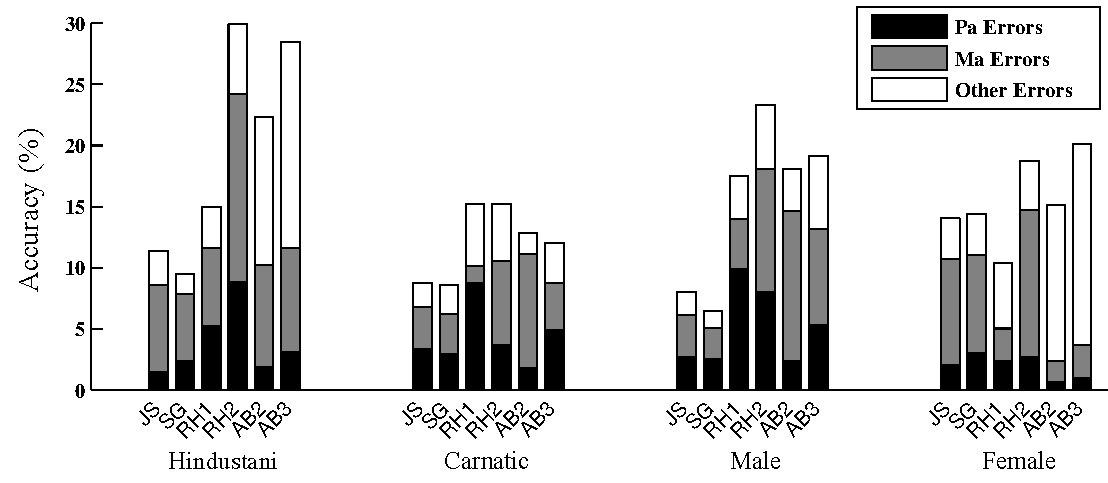
\includegraphics[width=\figSizeHundred]{ch05_preprocessing/figures/Category_Errors.pdf}
	\end{center}
	\caption[Percentage of Pa, Ma and `Other' type errors in tonic identification for different categories]{The percentage of audio excerpts with the different categories of errors (Pa, Ma and Others) for every method as a function of different excerpt attributes (Hindustani, Carnatic, male, female). Only the subscript in the names of the methods is used for labeling the axis.}
	\label{fig:tonic_identification_categorywise_errors}
\end{figure}

Finally, we analyze the errors as a function of the different attributes of the excerpts (Hindustani versus Carnatic, male versus female). As in~\secref{sec:pre_processing_tonic_id_results_only_audio_data}, we use the \acrshort{tds_cm2} dataset for this analysis because it is the most balanced dataset in terms of these attributes. Note that the methods are not provided with any metadata in addition to the audio signal. The percentage of excerpts containing each of the three categories of errors (Pa, Ma and Other) for every approach as a function of the different excerpt attributes is shown in ~\figref{fig:tonic_identification_categorywise_errors}. We see that for the classification-based methods, the proportion of Ma errors is much higher in performances by female singers compared to performances by male singers. The pitch range of the tonic for female singers is such that the lower Ma resides in the frequency range where the tonic of most male singers lies. Thus, the lower Ma-middle Sa (fifth) relationship for female singers is often confused with middle Sa-Pa relationship for male singers, resulting in a high number of Ma errors. For further details and insights regarding the types of error made by the
different methods and their underlying causes we refer the reader to the publications where these methods are discussed in depth \citep{salamon2012multipitch, SGulati_MThesis2012,bellur2012knowledge,ranjani2011carnatic}.


\subsection{Summary of the Comparative Evaluation }
\label{sec:pre_processing_tonic_identification_summary}

We evaluated seven tonic identification methods on six different and diverse datasets of \gls{iam}. The evaluation was performed in two scenarios: first, when only audio data is used as input to the methods, and second, when the additional information about the gender of the singer (male or female) and the performance type (vocal or instrumental) is given in addition to audio data. The results obtained are analyzed per dataset, and for different characteristics of the music material. Along with the accuracies of the methods, we presented an in-depth error analysis, describing the different kinds of errors for different scenarios and provided plausible explanations for them.

Overall, we see that methods \acrshort{tonicid_justin} and \acrshort{tonicid_sankalp} that use multipitch-based audio feature and classification methodology for selecting tonic pitch perform better than the rest. Their performance is better on all but one datasets considered in the evaluation (the exceptional dataset is small in size and contains poor quality audio recordings). In addition, the performance of these two methods appears to be the most consistent across music traditions, gender of the singer (male or female) and type of music performance (vocal or instrumental). 

Finally, we select \acrshort{tonicid_justin} method to identify tonic pitch from audio recordings in all the studies conducted as a part of this thesis. \acrshort{tonicid_justin} produces comparable results to \acrshort{tonicid_sankalp} and is relatively simpler to implement owing to a single stage processing. Furthermore, \acrshort{tonicid_justin} does not require any estimate of the predominant pitch, which makes it independent of the performance of the pitch estimation algorithms. The are two implementations of this method, which we make publicly available online~(\appref{app:resources}).


\subsection{Correcting Common Errors in Tonic Identification}
\label{sec:pre_processing_tonic_identification_correcting_errors}

As mentioned above, identification of the tonic pitch is a crucial first step required for nearly all meaningful melodic analyses of \gls{iam}. Any error in this step propagates through the processing chain and adversely affect the output of the melodic analyses. Though the accuracy of the most successful tonic identification method is nearly 90\% (\tabref{tab:tonic_identification_accuracy_without_gender_info}), even a 10\% error in tonic pitches can deteriorate the performance of melodic analyses described in the subsequent chapters. Moreover, it leads to an uncertainty, whether an error in the final output is caused due to a wrong tonic pitch or it is because of an error made in the later stages of the methods. 

We here present an heuristic-based approach to correct frequently occurring errors in tonic identification. From \tabref{fig:tonic_identification_errors_without_MF}, we see that the majority of the errors are Ma and Pa errors. Also, we know from the music knowledge that the tonic pitch chosen by the lead performers in \gls{iam} does not change drastically over the years and it typically remains within two semitones (200\,Cents). Since the accuracy of the tonic identification is nearly 90\%, for the recordings of an artist in our music corpus there might only be a handful of recordings for which the tonic values are incorrectly identified. Moreover, these wrong estimates are either Ma or Pa. These errors typically correspond to a pitch value that cannot possibly be the true tonic of the singer. Thus, these erroneous cases can be automatically detected by employing a majority voting. Once detected, the wrongly estimated tonic values can be transposed (either by fifth, or fourth) to match the most frequent tonic value of that artist in the corpus. After we perform this step, we achieve close to perfect tonic estimates for the music collection. %As can be imagined, this approach would work for artists that have more than a certain number of recordings in the collection. Since the recordings are ripped from the complete CDs, most of the artists considered in the datasets do have reasonable number of recordings in our corpus.


\section{Melody Processing}
\label{sec:data_preprocessing_melody_processing}

In this section, we present all the procedures applied in relation to the extraction and processing of a melody representation from raw audio signals. These processing steps can be grouped into three main categories: predominant pitch estimation (sometimes also referred to as predominant melody extraction), pitch post-processing, and melody representation. All these three steps are described at length in the subsequent sections. 

\begin{figure}
	\begin{center}
		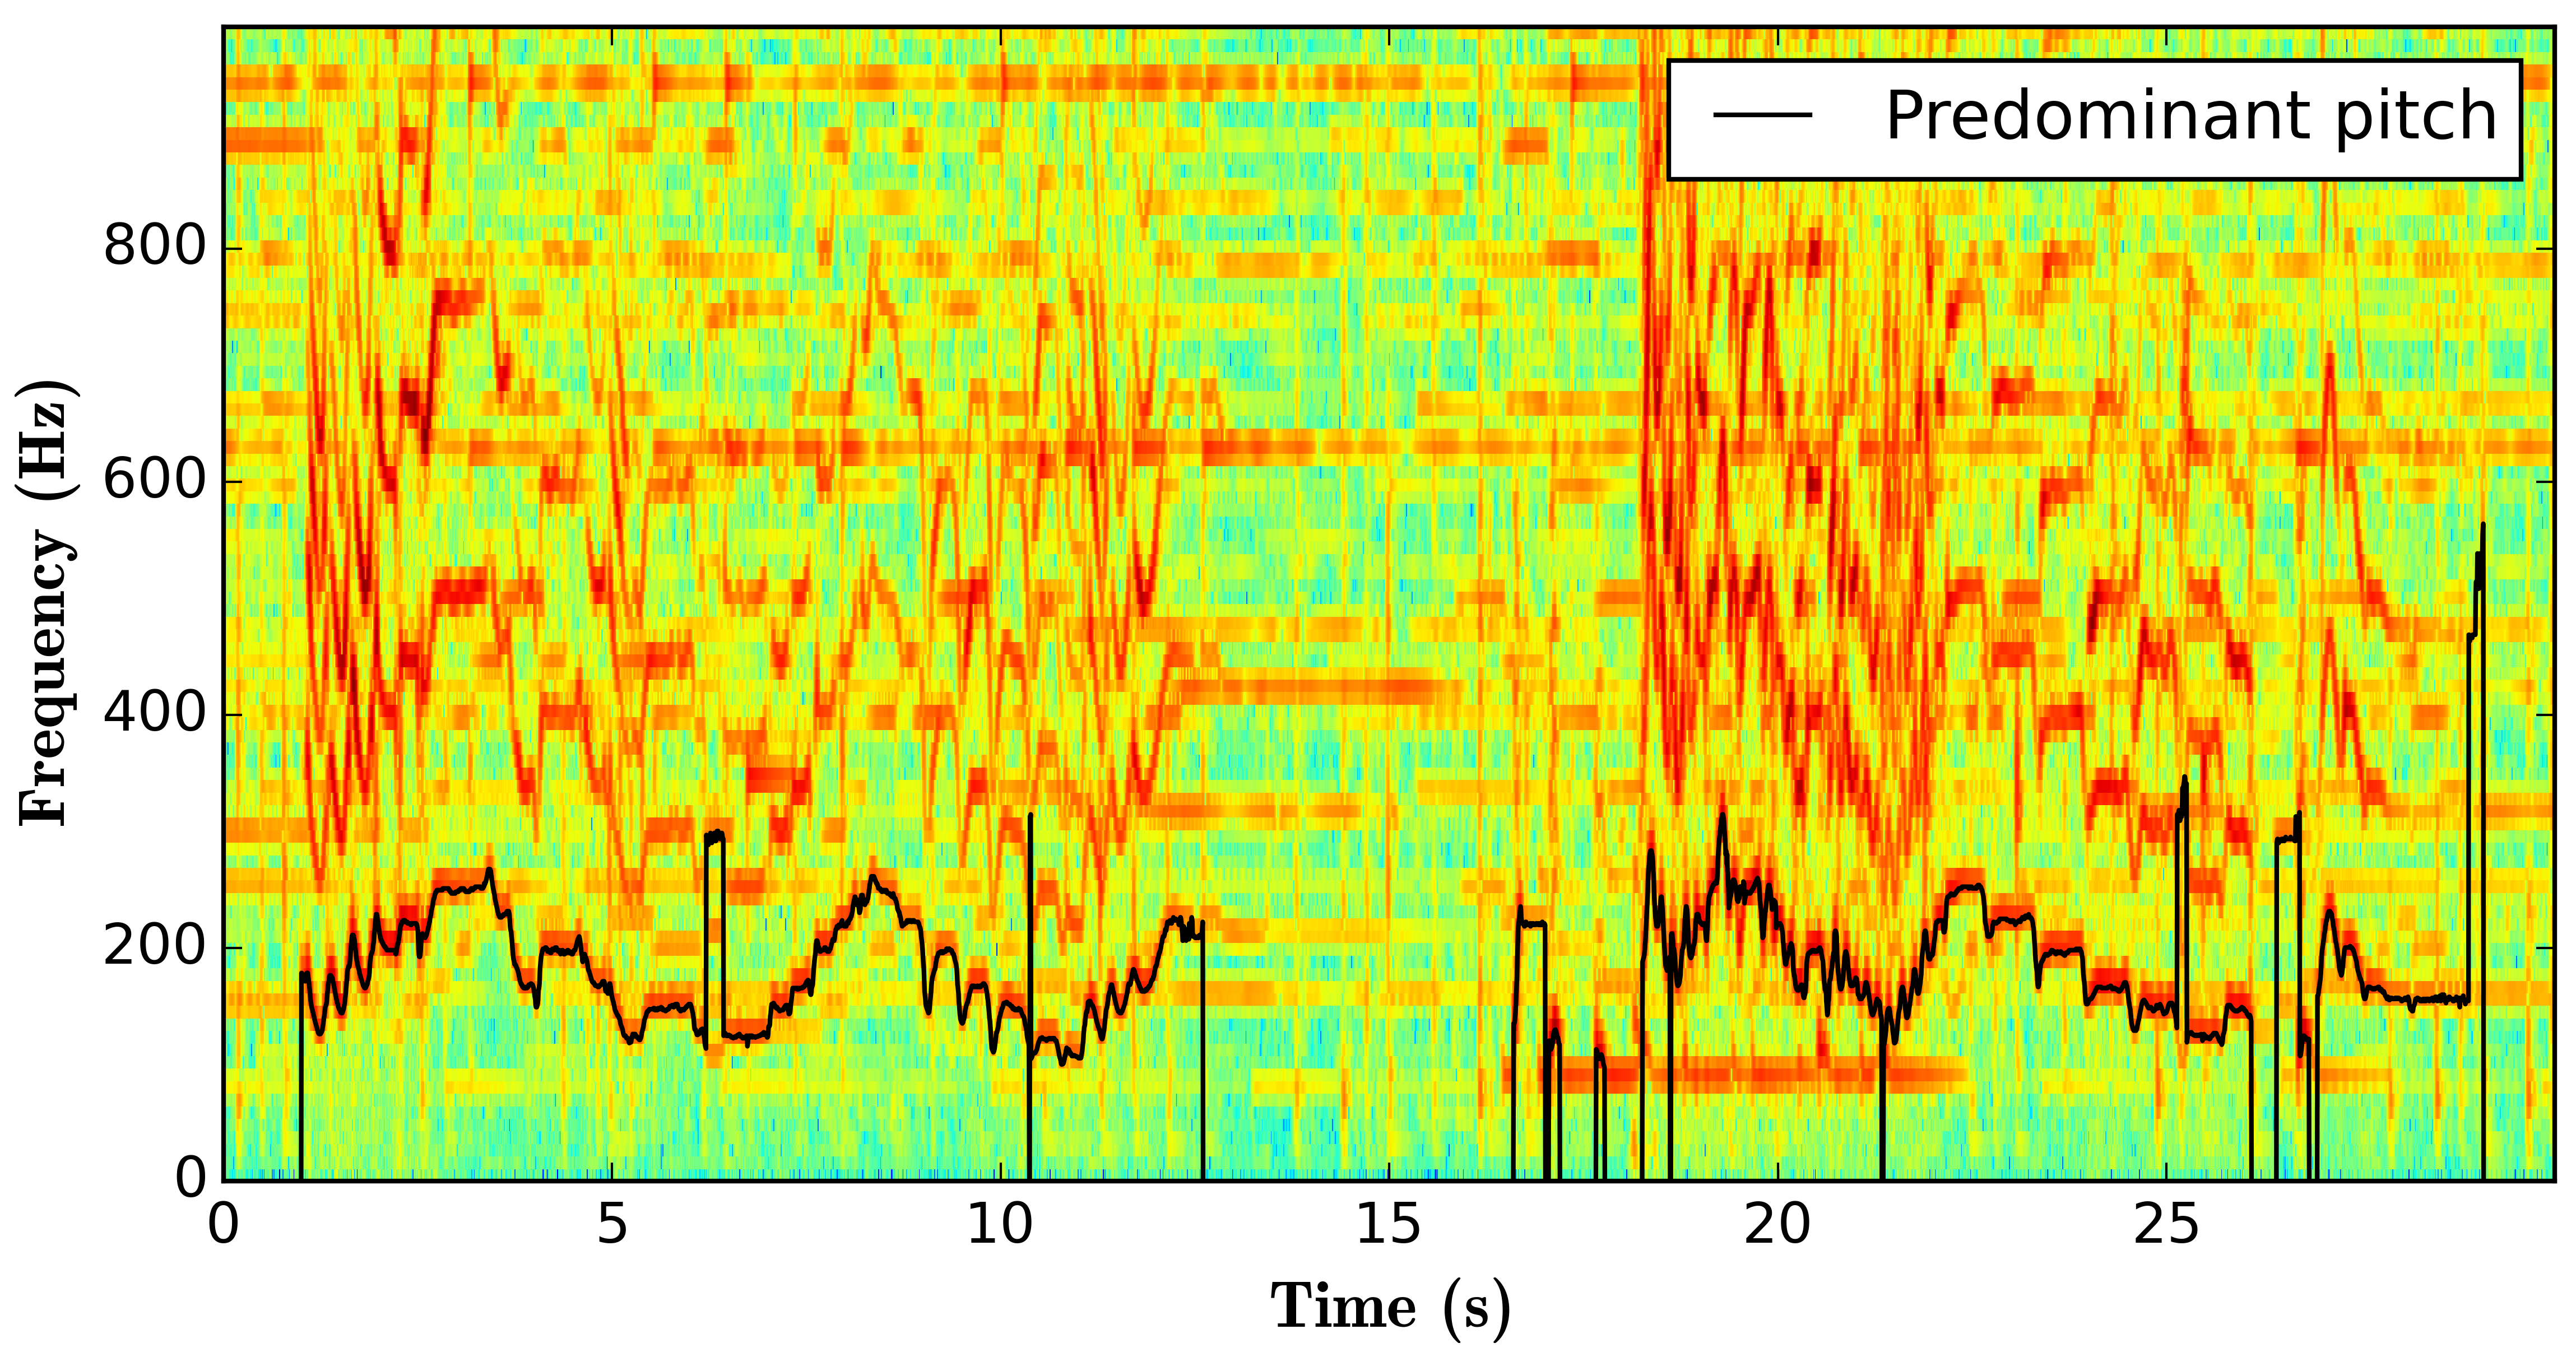
\includegraphics[width=\figSizeHundred]{ch05_preprocessing/figures/predominantMelodyExample.png}
	\end{center}
	\caption[Example of the predominant pitch representation of melody]{Example of a continuous pitch contour corresponding to the predominant melodic source extracted from a polyphonic audio excerpt.}
	\label{fig:predominant_melodic_fragment}
\end{figure}


\subsection{Predominant Pitch Estimation}
\label{sec:data_preprocessing_predominant_melody_estimation}

In \secref{sec:background_terminology}, we presented our working definition of melody. In a nutshell, we consider the continuous pitch contour corresponding to the predominant melodic source (typically, the lead artist) in the audio recording as the low-level representation of melody. An example is shown in~\figref{fig:predominant_melodic_fragment}, wherein the contour represents the pitch of the lead singer at each instance in time. Usage of such a melody representation is a common practice in \gls{mir}, and is done for a variety of melody processing tasks across different music traditions~\citep{Dutta2014,Ishwar2013,Rao2014,koduri2014intonation,senturk2013score,pikrakis2012tracking,pikrakis2003recognition,moelants2009exploring}. 

Pitch estimation, also commonly known as pitch tracking from audio signals has been an active research topic since several decades~\citep{salamon:phd:13}. The challenges in the estimation of a reliable pitch contour differ across the type of audio music signals (monophonic or polyphonic). As a result of which the performance of these algorithms vary significantly across different music genres, which also seems to be correlated with the extent of the polyphony in the music. A sparse polyphonic characteristic in audio recordings of \gls{iam} due to its heterophonic nature lessens the complexity of the task to an extent, when compared to several other western popular music genres. This trend is clearly visible from the past MIREX (an international MIR evaluation campaign) results\footnote{\url{http://www.music-ir.org/mirex/wiki/MIREX_HOME}}. For example, compare the accuracy obtained by different algorithms on INDIAN08\footnote{\url{http://nema.lis.illinois.edu/nema_out/mirex2011/results/ame/indian08/summary.html}},  MIREX05\footnote{\url{http://nema.lis.illinois.edu/nema_out/mirex2011/results/ame/mirex05/summary.html}} and  MIREX09~0dB\footnote{\url{http://nema.lis.illinois.edu/nema_out/mirex2011/results/ame/mirex09_0dB/summary.html}} datasets from MIREX-2011. 

In order to estimate the predominant pitch (denoted hereafter by $\pitchHz$) in the audio recordings of \gls{iam} we use \gls{melodia} algorithm, a state-of-the-art melody extraction method proposed by~\cite{Salamon2012}. This method performed favorably in MIREX~2011 on a variety of music genres, including \gls{iam}\footnote{\url{http://nema.lis.illinois.edu/nema_out/mirex2011/results/ame/indian08/summary.html}}. This method is used in several other studies that analyze melodies extracted from audio signals~\citep{Dutta2014,Ishwar2013,Rao2014,koduri2014intonation,senturk2013score,pikrakis2012tracking}.

Another motivation to use this algorithm is that it works on continuous pitch contours and employs auditory streaming constraints to ensure a continuity in the output pitch. As a result of this processing, it does not produce octave errors at the frame-level. Noticeably, this predominant pitch estimation algorithm also performs voicing detection. This means that the algorithm in addition to estimating the predominant pitch also detects the time segments where the voice is absent. %Such time segments where the predominant melodic source is inactive are assigned a dummy pitch value (usually 0).

Currently, there are two implementations of \gls{melodia} algorithm that are publicly available. We use its implementation as available in \Gls{essentia}~\citep{essentia}. \Gls{essentia}\footnote{https://github.com/MTG/essentia} is an open-source C++ library for audio analysis and content-based MIR. We use the default values of the parameters, except for the frame and hop sizes, which are set to 46 and 2.9\,ms, respectively. The other implementation of \Gls{melodia} is available as a Vamp plug-in\footnote{http://mtg.upf.edu/technologies/melodia}. 

Prior to the predominant pitch estimation we apply an equal-loudness filter\footnote{\url{http://wiki.hydrogenaud.io/index.php?title=ReplayGain_1.0_specification}} to make the processing perceptually relevant~\citep{essentia}. For this operation as well we use Essentia with the default values of the parameters. 

In every computational task addressed in this thesis we use the \Gls{melodia} algorithm to estimate the predominant pitch for all the datasets. There is only one exception, \acrshort{msds_iitb_hmd} dataset, which was introduced in~\cite{Ross2012b} for computing melodic similarity. \acrshort{msds_iitb_hmd} dataset along with audio recordings and melodic phrase annotations also includes semi-automatically extracted predominant pitch contours~(\secref{sec:corpus_melodic_similarity_dataset}). Using the pitch contours provided along with the dataset allows us to compare the output of our method with other studies. In addition, since these pitch contours are nearly free from any octave errors, we avoid propagating errors to subsequent stages, and thus, evaluate the task of melodic similarity more reliably. 

In our work in this thesis we consider only the pitch dimension of melody in its representation. However, loudness and timbral dimensions of melody that largely capture the phonetics and expressive aspects are also informative and can be helpful in several tasks including computation of melodic similarity. To give an idea about the type of information captured in the loudness and timbral dimensions and their usefulness, we take an example. We synthesize the harmonic series corresponding to a voice extracted from an excerpt of Carnatic music. During the synthesis we force the pitch of the voice to a monotone while keeping the other aspects (loudness and timbre) intact. The original excerpt\footnote{\url{http://www.freesound.org/people/sankalp/sounds/352810/}}, synthesized predominant pitch\footnote{\url{http://www.freesound.org/people/sankalp/sounds/352809/}} and the synthesized monotone voice\footnote{\url{http://www.freesound.org/people/sankalp/sounds/352808/}} is made available for listening. After listening to this example, we get an idea about the nature of the melodic characteristics that are not utilized if we only consider the pitch dimension of melody in the analysis. Exploiting loudness and timbral dimensions for melodic analysis shall be taken up in the future endeavors.


\subsection{Pitch Post-processing}
\label{sec:data_preprocessing_pitch_postprocessing}

Predominant pitch estimation in polyphonic audio recordings has not been solved yet, and the output pitch contour is still far from being perfect (MIREX-2011 results\footnote{\url{http://nema.lis.illinois.edu/nema_out/mirex2011/results/ame/indian08/summary.html}}, MIREX-2016 results\footnote{\url{http://nema.lis.illinois.edu/nema_out/mirex2016/results/ame/ind08/summary.html}}). While these algorithms get better over years, a number of errors in the predominant pitch estimation can be alleviated by post-processing the pitch contour. In post-processing, our main objective is to correct the spurious pitch octave jumps and smoothen the extracted pitch contour. In addition, for certain tasks described in the subsequent chapters, we also interpolate the unvoiced regions in the melody that correspond to the short-duration breath pauses taken by the artists. We now describe these post-processing steps in detail.

\subsubsection{Correcting Spurious Pitch Jumps}
\label{sec:data_processing_correcting_pitch_jumps}

\begin{figure}
	\begin{center}
		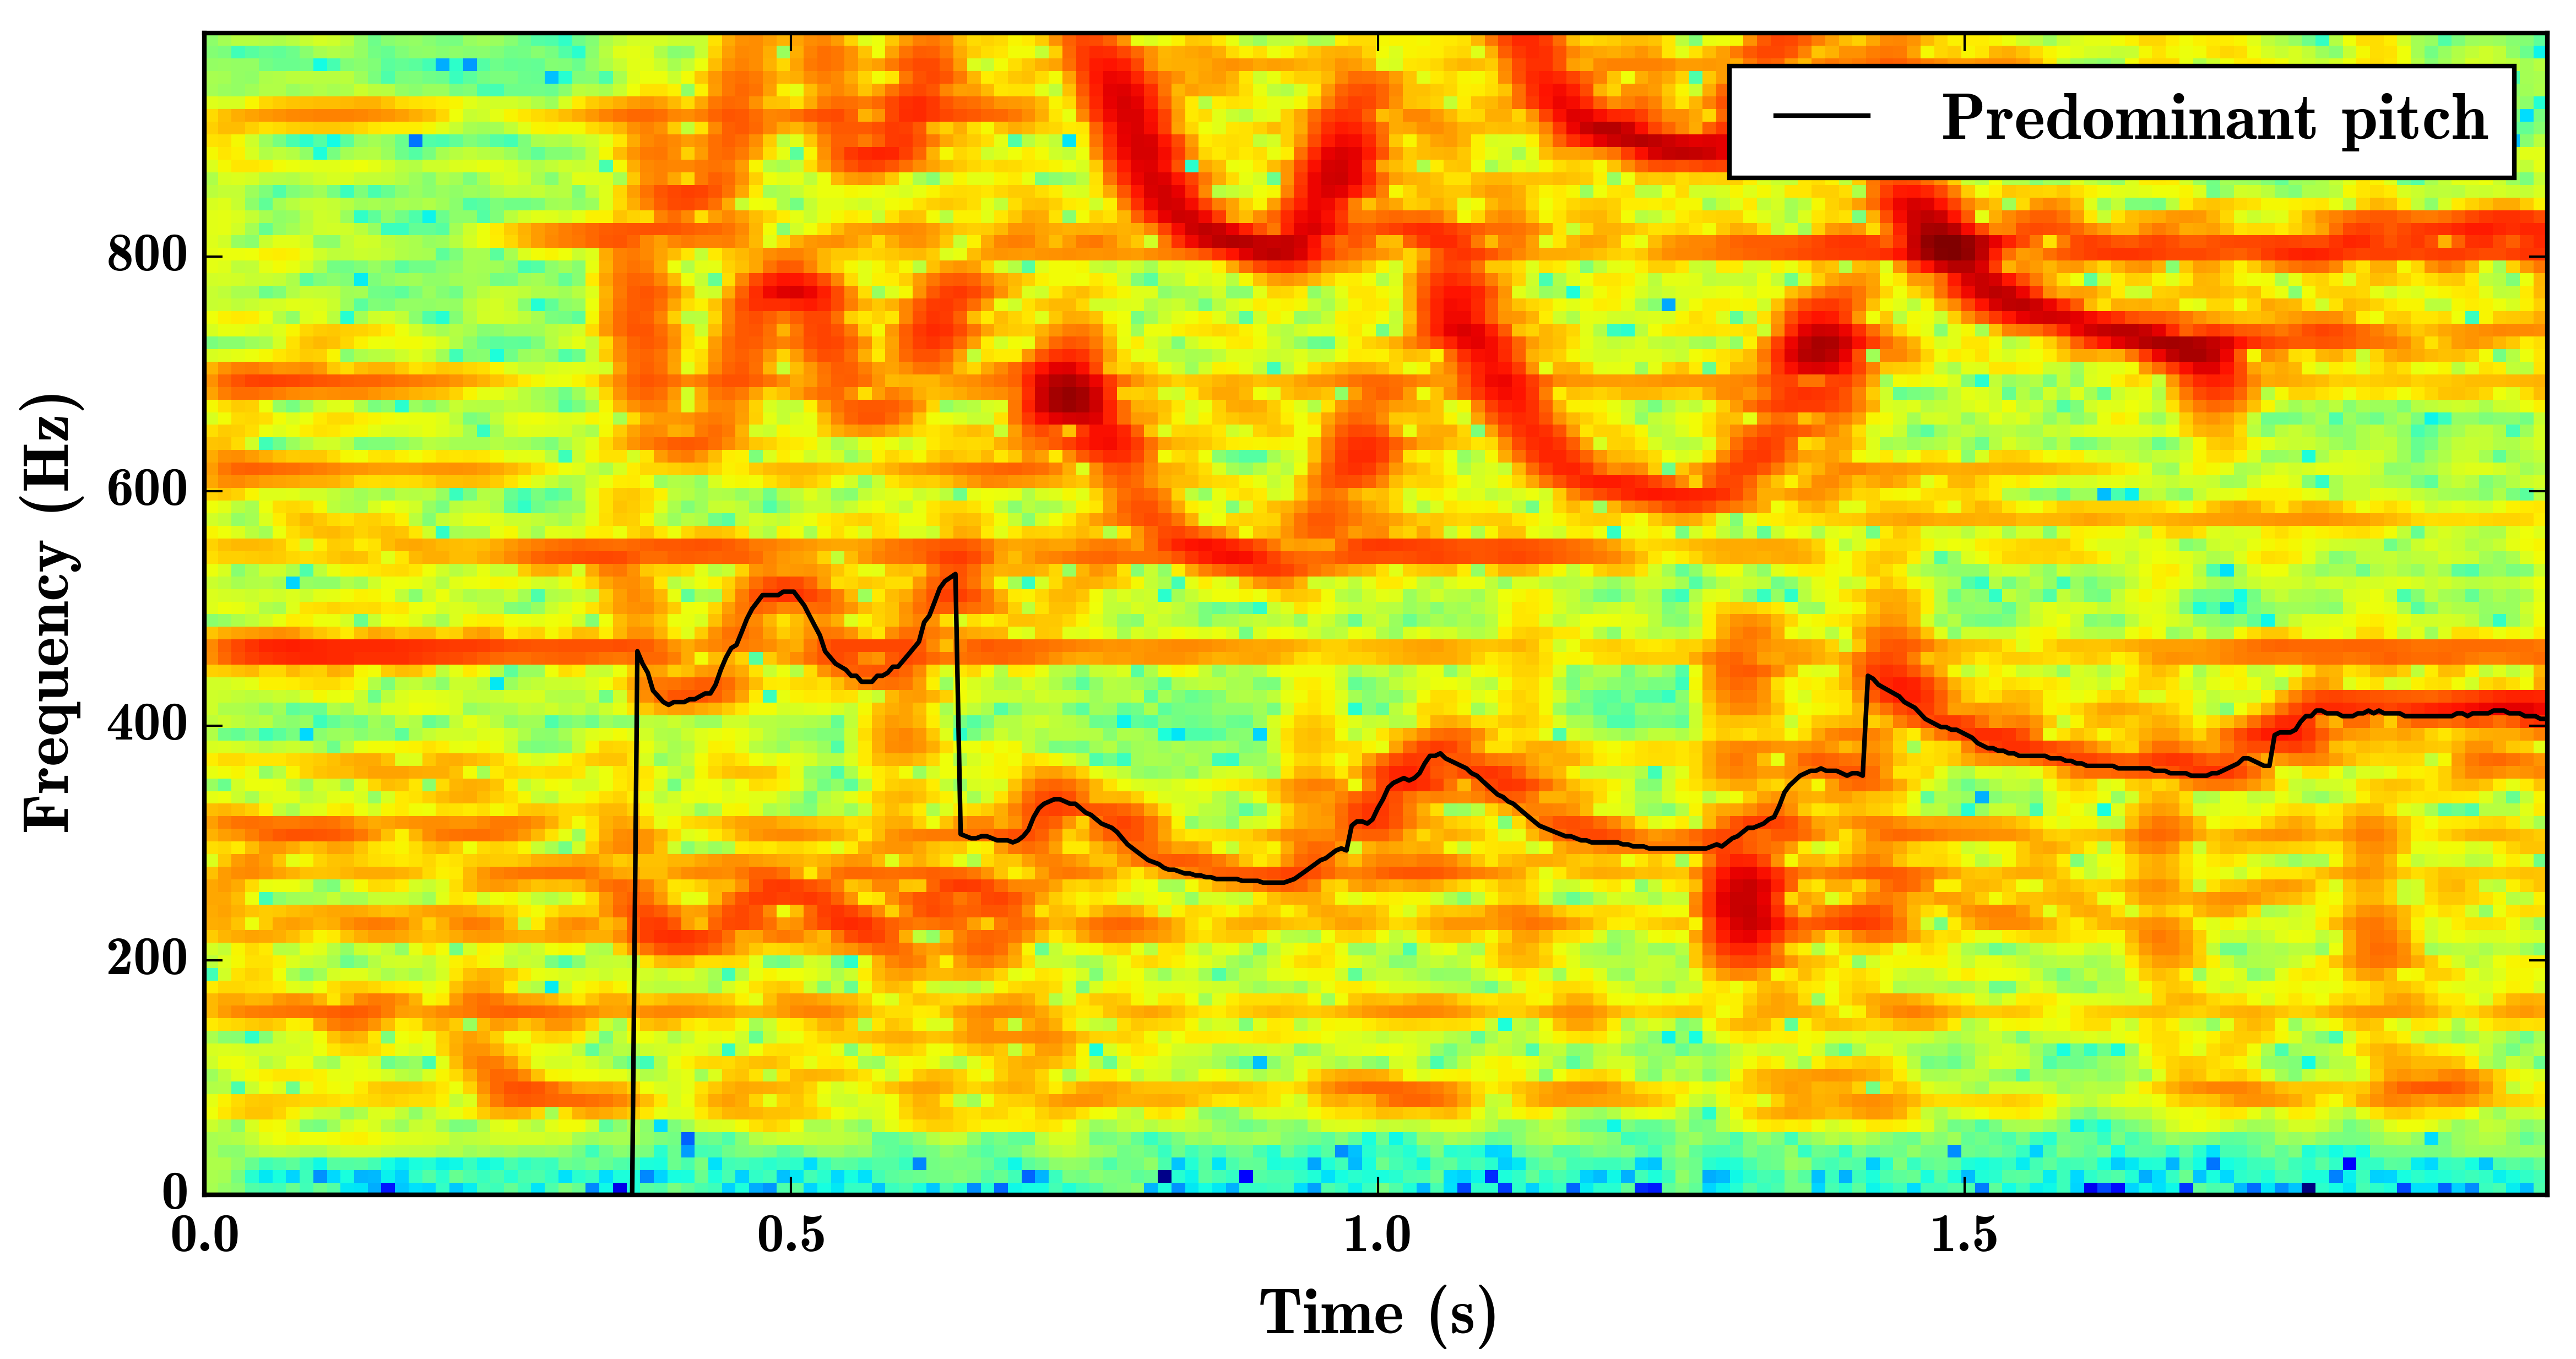
\includegraphics[width=\figSizeHundred]{ch05_preprocessing/figures/octaveErrorIllustration.png}
	\end{center}
	\caption{Example of an octave error in predominant pitch contour.}
	\label{fig:octave_error_pitch}
\end{figure}

One of the most frequently occurring errors in pitch estimation is it's detecting in a wrong octave, commonly referred to as an octave error. Identifying and correcting such errors during a post-processing step for the case of a monophonic signal (containing a single harmonic series) is fairly simple. One can compare the energy of the partials with the total energy of the audio frame to infer if the estimated pitch value corresponds to the actual fundamental frequency. However, in the case of a polyphonic music signal it becomes a challenging task. 

We alleviate this problem to an extent by restricting ourselves to a specific type of pitch octave error occurring over a short duration of time. Instead of identifying an octave error for an individual audio frame, we exploit the temporal melodic continuity to detect such errors. We explain the intuition behind our method with the help of an example shown in~\figref{fig:octave_error_pitch}. If we analyze an isolated audio frame at 0.5\,s, identifying a pitch octave error computationally becomes a challenging task. However, by analyzing the pitch continuity we can easily detect an anomalous pitch jump of roughly 1200\,cents at time 0.65\,s. This is due to the fact that such drastic pitch jumps across frames do not occur naturally in singing voice. By analyzing the amount of frequency difference across the pitch transition we can infer to an extent the type of pitch error and can subsequently correct it. Since the detected pitch jump is around 1200\,cents, it is highly likely to be an octave error. In this example voice starts at around 0.4\,s, which we consider as a positive pitch jump. Knowing that there is a anomalous pitch jump in the other direction (negative pitch jump) at time 0.65\,s makes it highly probable that the pitch segment between time 0.4\,s and 0.65\,s suffers from an octave error.  

We describe this heuristic-based approach in~\algoref{alg:algorithmPitchCorrection}. In this algorithm $\mathrm{winSize}$ is set to 1\,s and $\mathrm{silenceCentValue}$ is set to $1200*\log2(\epsilon)$, where $\epsilon$ is of the order of $10^{-17}$.


\renewcommand{\algorithmiccomment}[1]{\bgroup\hfill\tiny//~#1\egroup}

\begin{algorithm}
	\caption{Correcting spurious pitch octave jumps}
	\label{alg:algorithmPitchCorrection}
	\begin{algorithmic}  
		\State {\bf Input:} pitch sequence ($\pitchHz$) of length N samples in Cents scale
		\State jumpType = zeros(N)	
		
		\For{ii=0; ii<N; ii++}							\Comment{Detecting type of pitch transition}
		\State diff = $\pitchHz$[ii+1]-$\pitchHz$[ii]
		\If{abs(diff)\%1200 <= 300}
		\If {diff > 0}
		\State jumpType[ii+1]=3			\Comment{Positive octave jump}
		\ElsIf {diff<0}
		\State jumpType[ii]=4			\Comment{Negative octave jump}
		\EndIf
		\ElsIf {abs(diff)>=600}
		\If {$\pitchHz$[ii]= silenceCentValue}
		\State jumpType[ii+1]=1			\Comment{Unvoiced to voiced}
		\ElsIf {$\pitchHz$[ii+1]= silenceCentValue}
		\State jumpType[ii]=2			\Comment{Voiced to unvoiced}
		\ElsIf {diff>0}
		\State jumpType[ii+1]=5			\Comment{Other positive pitch jump}
		\Else
		\State jumpType[ii]=6			\Comment{Other negative pitch jump}
		\EndIf
		\EndIf
		\EndFor
		
		\For {ii=0; ii<N-winSize; ii++}				\Comment{Fixing pitch octave jumps}
		\State shift = 0
		\State indJumps = where(jumpType[ii:ii+winSize]!=0)			
		\If {len(indJumps) == 2}				\Comment{Process only when two jumps are detected}
		\State i1 = indJumps[0] + ii
		\State i2 = indJumps[1]	+ ii			
		\If {jumpType[i1] + jumpType[i2] == 3}		
		\State jumpType[i1] = 0
		\State continue			\Comment{Do nothing for unvoiced to voiced to unvoiced}
		\EndIf
		
		\If {jumpType[i1]\%2 = 1 and jumpType[i2]\%2 = 0 }
		\If {jumpType[i1] == 3 and jumpType[i2] != 6}
		\State shift = 1200*round((p[i1] - p[i1-1])/1200)
		\ElsIf {jumpType[i2] == 4 and jumpType[i1] != 5}
		\State shift = 1200*round((p[i2] - p[i2+1])/1200)
		\ElsIf {jumpType[i1] == 1}
		\State shift = 100*round((p[i2] - p[i2+1])/100)
		\ElsIf {jumpType[i2] == 2}
		\State shift = 100*round((p[i1] - p[i1-1])/100)
		\EndIf
		\EndIf
		\EndIf
		\State $\pitchHz$[i1:i2+1] = $\pitchHz$[i1:i2+1] - shift
		\State jumpType[i1] = 0
		\State jumpType[i2] = 0		
		
		\EndFor
		
	\end{algorithmic}
\end{algorithm}


\subsubsection{Pitch Smoothening}
\label{sec:data_processing_pitch_smoothening}


\begin{figure}
	\begin{center}
		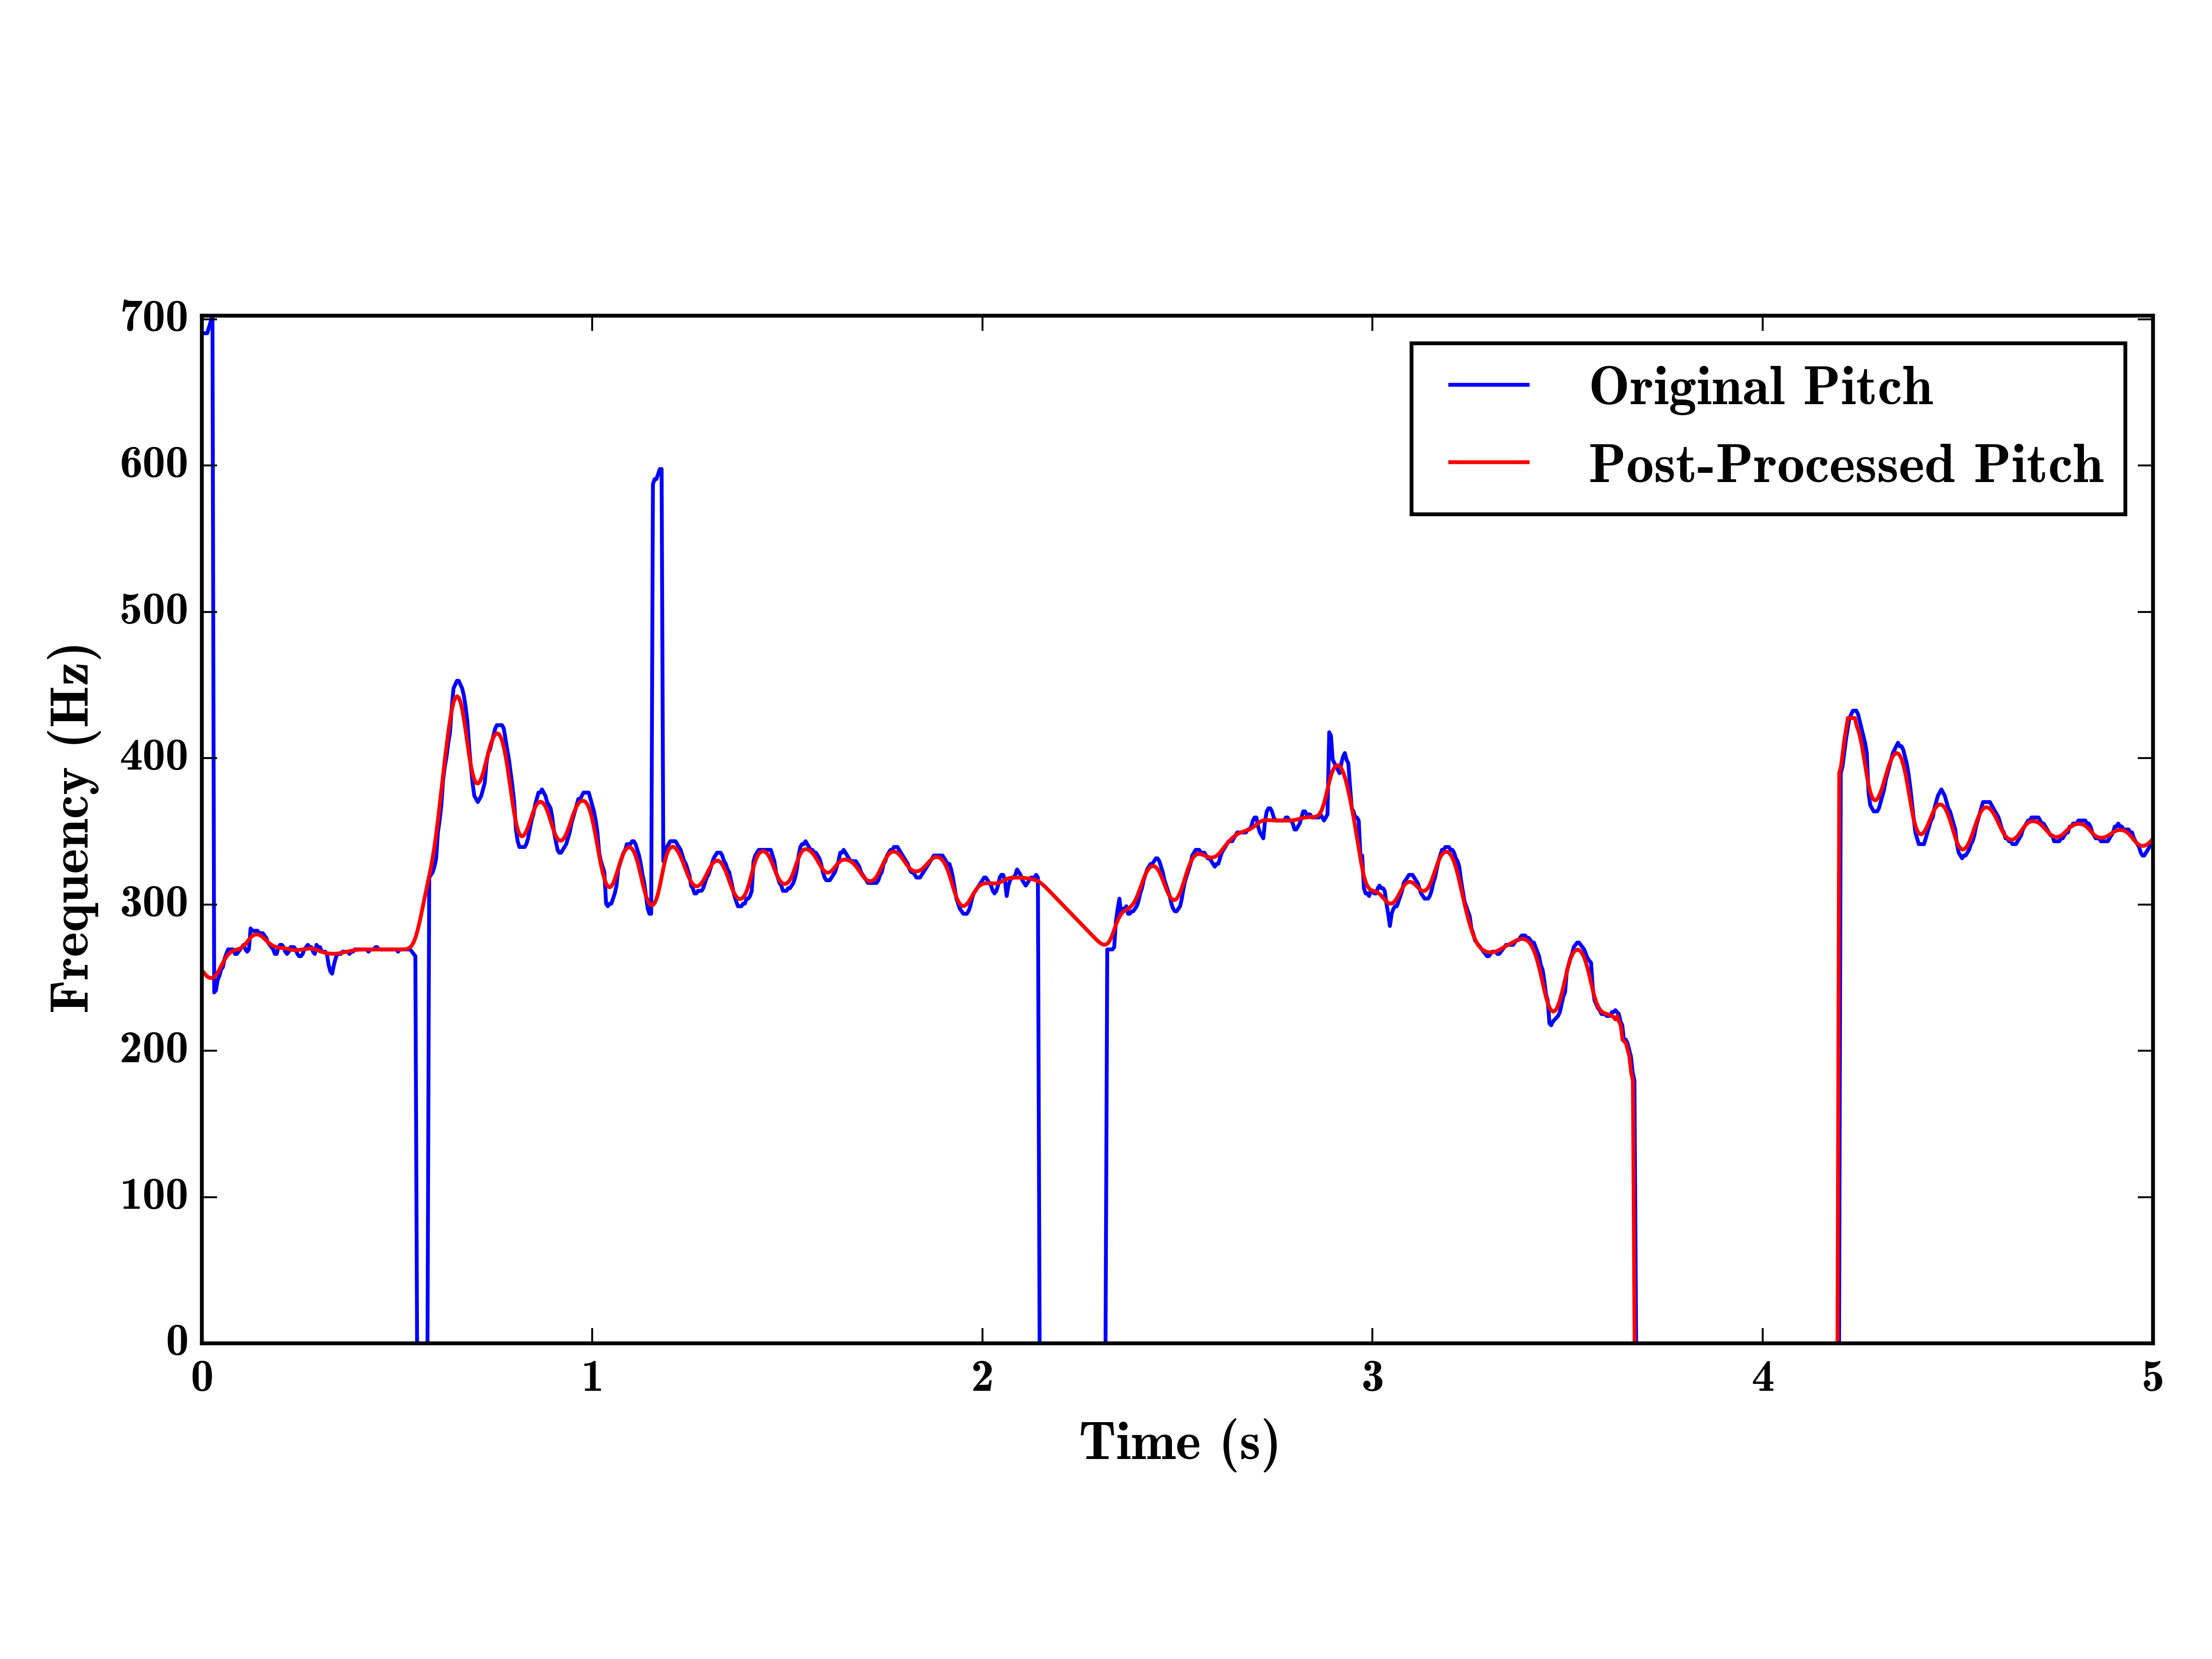
\includegraphics[width=\figSizeHundred]{ch05_preprocessing/figures/smootheningExample.png}
	\end{center}
	\caption[Example of a post-processed predominant pitch segment]{Example of a pitch segment before and after post-processing, which involve median filtering, Gaussian filtering and interpolation of the short unvoiced regions.}
	\label{fig:smoothening_example}
\end{figure}

This processing step aims to remove the spurious pitch jumps lasting over a few frames and to smooth the pitch contours. We start by performing a median filtering on the estimated pitch contour. The window length chosen for median filtering is 50\,ms. Subsequently, to smooth the pitch contour we apply a low-pass filtering by using a Gaussian window. The window size and the standard deviation of the Gaussian window is set to 50\,ms and 10\,ms, respectively. In~\figref{fig:smoothening_example} we show an example of a pitch segment before and after applying median filtering and Gaussian smoothening. We see that the spurious pitch jumps are removed and the pitch contour appears smooth.


\subsubsection{Pitch Interpolation}
\label{sec:data_processing_pitch_interpolation}

In the rendition of melodic phrases in \gls{iam}, there are often unvoiced segments lasting over a small time interval. These unvoiced segments may either correspond to short breath-pauses taken by the vocalists or to the consonants in the lyrics, which are unvoiced in nature. These short unvoiced segments pose a difficulty in the computation of melodic similarity since they do not exist in all the occurrences of a melodic phrase. In such situations assignment of a meaningful numerical value to these unvoiced melodic regions is desired. Therefore, in order to avoid the complexities arising from these unvoiced melodic segments, we interpolate these regions. We perform a linear interpolation across all the unvoiced segments that last for less than 300\,ms. An example of an interpolated unvoiced segment is shown in~\figref{fig:smoothening_example}, between time range of 0 to 1\,s, and 2 to 3\,s.

\subsubsection{Pitch Resampling}
\label{sec:data_processing_pitch_resampling}

An optimal sampling rate of the predominant pitch might depend on the particular computational task under study. For tasks such as analysis of melodic ornaments in \gls{iam}, a high sampling rate might be desired, whereas, for computationally complex tasks such as melodic pattern discovery and search, a sampling rate as low as possible but sufficient to capture melodic nuances might be preferred. In order to avoid predominant melody computation for different sampling rates used across experiments, we resample the predominant melody contours extracted once at a high sampling rate. Pitch contours are decimated to a lower sampling rate by simply downsampling them by an integer factor. The downsampling factor is decided based on the sampling rate used in a particular experiment.

Note that, not all the post-processing steps described in this section are employed in all the experiments. The description of the specific methods in the subsequent chapters will contain details about the post-processing steps used in their respective experiments.


\subsection{Melody Representation} 
\label{sec:pre_processing_melody_representation}

\subsubsection{Hertz to Cent Conversion}
\label{sec:data_processing_cent_conversion}

The perception of melodic intervals for human beings is logarithmic in nature with respect to pitch (or fundamental frequency in Hz). Thus, in order for the pitch representation to be musically meaningful, we convert the estimated predominant pitch values from Hertz to Cents (logarithmic scale) following the equation below.

\begin{equation}
\label{eq:hertz_to_cent_conversion}	
\pitchCents_i = 1200~\log_2\left(\frac{\pitchHz_i}{f_r}\right) ,
\end{equation}

\noindent where $\pitchHz_i$ is the $i^\mathrm{th}$ sample of the predominant pitch in Hertz-scale, $\pitchCents_i$ is the $i^\mathrm{th}$ sample of the predominant pitch in Cent-scale, $f_r$ is the reference tuning frequency which typically in the case of western popular (or even classical) music is set to an integer multiple or sub-multiple of 440\,Hz. We consider $f_r=55$\,Hz, although as we will notice in the next section that this choice is inconsequential.
  

\subsubsection{Tonic Normalization}
\label{sec:tonic_normalization}

As described in~\secref{sec:melody_in_iam} and in~\secref{sec:data_preprocessing_tonic_identification}, in a performance of \gls{iam}, the tonic pitch of the lead performer serves as the reference frequency. Every lead artist chooses a tonic pitch, using which the \gls{tanpura} and the rest of the instruments are tuned. To analyze a melody in the tonal context established by the tonic pitch in a recording ($\toniRec$), we normalize the predominant pitch by this frequency. We perform this normalization by considering the reference frequency $f_r=\toniRec$ in \eqnref{eq:hertz_to_cent_conversion}, which is estimated for every recording using \acrshort{tonicid_justin} method~(\secref{sec:pre_processing_tonic_identification_summary}).


\section{\titlecap{\glsentrytext{nyas} \glsentrytext{svara} Segmentation}}
\label{sec:pre_processing_nyas_segmentation}

Musical melodies contain hierarchically organized events that follow a specific grammar~\citep{Patel07BOOK}. Some of these events are musically more salient than others and act as melodic landmarks. Cadential notes in classical Western music~\citep{GroveCadence} or \gls{karvai} regions in Carnatic music~\citep{sambamoorthy:1998} are examples of such landmarks. While some of these landmarks can be identified based on a fixed set of rules, others do not follow any explicit set of rules and are learned implicitly by a musician through years of music training. A computational analysis of these landmarks can discover some of these implicitly learned rules and help in developing musically aware tools for music exploration, understanding and education. 

Occurrence of a \gls{nyas} in Hindustani music melodies is an example of such a melodic landmark that we investigate in this section. A detailed description of \gls{nyas} is provided in \secref{sec:melody_in_iam}. Typically, occurrence of a \gls{nyas} delimits melodic phrases, which constitute one of the most important characteristic of a \gls{raga}. Analysis of \gls{nyas} is thus a crucial step towards the melodic analysis of Hindustani music. In particular, automatically detecting occurrences of \gls{nyas} (from now on referred as \gls{nyas} segments) will aid in melody segmentation, which is a crucial step in melodic phrase discovery. However, detection of \gls{nyas} segments is a challenging computational task, as the prescriptive definition of \gls{nyas} is very broad, and there are no fixed set of explicit rules to quantify this concept~\citep[p. 73]{Dey2008}. It is through rigorous practice that a seasoned artist acquires perfection in the usage of \gls{nyas}, complying with the \gls{raga} grammar and exploring creativity through improvisation at the same time. 


\begin{figure}
	\begin{center}
		\ifdefined\PRINTVER
			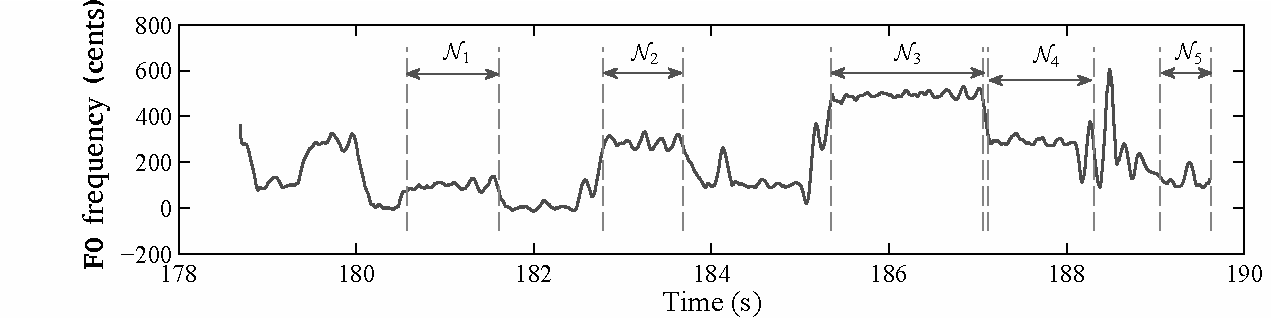
\includegraphics[width=\figSizeHundred]{ch05_preprocessing/figures/NyasFragmentChallenge_BW.pdf}
		\else
			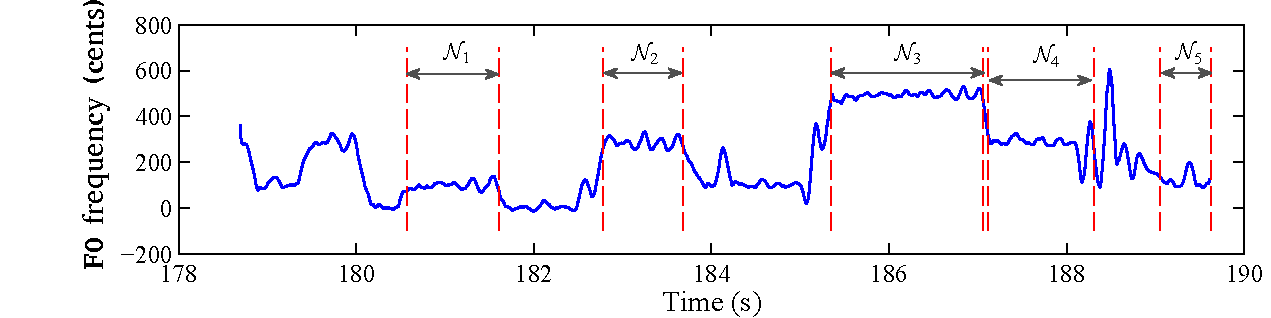
\includegraphics[width=\figSizeHundred]{ch05_preprocessing/figures/NyasFragmentChallenge.pdf}
		\fi
		
	\end{center}
	\caption[A fragment of a pitch contour showing \gls{nyas} segments]{A fragment of a pitch contour showing \gls{nyas} segments denoted by $\nSvara_i$ ($i={1...5}$).}
	\label{fig:nyas_segments_example}
\end{figure}

From a computational perspective, the detection of \gls{nyas} segments is challenging due to the variability in segment length, melodic characteristics and the different melodic contexts in which \gls{nyas} is rendered. To illustrate this point we show a fragment of pitch contour in~\figref{fig:nyas_segments_example}, annotated with \gls{nyas} segments denoted by $\nSvara_i$ ($i={1...5}$). We see that the \gls{nyas} segment length is highly varied, where $\nSvara_5$ is the smallest \gls{nyas} segment (even smaller than many non-\gls{nyas} segments) and $\nSvara_3$ is the longest \gls{nyas} segment. In addition, pitch contour characteristics also vary a lot due to the presence of \gls{alankar} (\secref{sec:melody_in_iam}). The pitch characteristics of a segment depend on the \gls{raga} and scale degree of the \gls{nyas}, and adds further complexity to the task~\citep{Bagchee1998}. For example, in~\figref{fig:nyas_segments_example}, $\nSvara_1$ and $\nSvara_3$ have a small pitch deviation from the mean \gls{svara} frequency, whereas, $\nSvara_2$ and $\nSvara_4$ have a significant pitch deviation (close to 100\,cents in $\nSvara_5$). Large pitch deviations also pose a challenge in segmentation process. Furthermore, melodic context such as the relative position with respect to a non-voiced or long melodically constant region plays a crucial role in determining a \gls{nyas} segment. Because of these factors the task of \gls{nyas} segment detection becomes challenging and requires sophisticated learning techniques along with musically meaningful domain specific features.

In the computational analysis of \gls{iam}, \gls{nyas} segment detection has not received much attention in the past. To the best of our knowledge, only one study with the final goal of spotting melodic motifs has indirectly dealt with this task~\citep{Ross2012}. In it, the authors considered performances of a single \gls{raga} and focused on a very specific \gls{nyas} \gls{svara}, corresponding to a single scale degree: the fifth with respect to the tonic, Pa \gls{svara}. This \gls{svara} is considered as one of the most stable \glspl{svara}, and has minimal pitch deviations. Thus, focusing on it oversimplified the methodology developed in~\cite{Ross2012} for \gls{nyas} segment detection. Note that the concept of landmark has been used elsewhere, with related but different notions and purposes. That is the case with time series similarity~\citep{Perng00ICDE}, speech recognition~\citep{Jansen08JASA,Chen12ICASSP}, or audio identification~\citep{Duong13ICASSP}.

In this section, we describe our method for detecting occurrences of \gls{nyas} \gls{svara} in Hindustani music melodies. The description is based on our work presented in~\cite{gulati2014Landmark}. The method consists of two main steps: segmentation based on domain knowledge, and segment classification-based on a set of musically motivated pitch contour features. There are three main reasons for selecting this approach over a standard pattern detection technique (for example \gls{dtw}). First, the pitch contour of a \gls{nyas} segment obeys no explicit patterns, hence, the contour characteristics have to be abstracted. Second, information regarding the melodic context of a segment can be easily interpreted in terms of discrete features. Third, we aim to measure the contribution of a specific feature in the overall classification accuracy (for example, if contour variance and length are the most important features for the classification). This is important in order to corroborate the results obtained from such data driven approaches with that from musicological studies. In the subsequent sections we first describe our method~(\secref{sec:pre_processing_nyas_id_method}), present the methodology used for evaluation~(\secref{sec:pre_processing_nyas_segmentation_experimental_setup}), discuss the results and summarize our findings~(\secref{sec:preprocessing_nyas_segmentation_results_and_discussion}).

\subsection{Method}
\label{sec:pre_processing_nyas_id_method}

The block diagram of the proposed method for \gls{nyas} segmentation is shown in~\figref{fig:bd_nyas_segmentation}. It consists of four main processing blocks: predominant pitch estimation and representation, segmentation, feature extraction, and segment classification and fusion. These processing blocks are described in the following sections.

\begin{figure}
	\begin{center}
		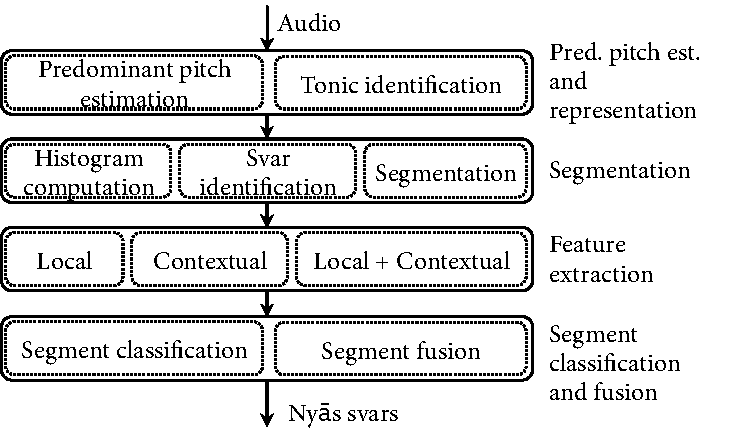
\includegraphics[width=\figSizeEightyFive]{ch05_preprocessing/figures/BlockDiagramNyasSegmentation.pdf}
	\end{center}
	\caption{Block diagram of the proposed approach for \gls{nyas} segmentation.}
	\label{fig:bd_nyas_segmentation}
\end{figure}

\subsubsection{Predominant Pitch Estimation and Representation}

To estimate pitch of the predominant melodic source we use the procedure described in~\secref{sec:data_preprocessing_predominant_melody_estimation} with the same set of parameters. We do not perform any post-processing on the estimated pitch contours. Pitch estimated in Hertz is converted to Cent-scale and is normalized by the tonic of the lead artist in the recording as described in~\secref{sec:data_processing_cent_conversion} and \secref{sec:tonic_normalization}. Tonic pitch of an audio recording is estimated using \acrshort{tonicid_justin} method~(\secref{sec:pre_processing_tonic_identification_summary}). 


\subsubsection{Segmentation}
\label{sec:nyas_svara_segmentation_method}

\Gls{nyas} segment is a rendition of a single \gls{svara} and the aim of the segmentation process is to detect the \gls{svara} boundaries. However, \glspl{svara} contain different \glspl{alankar}, where the pitch deviation with respect to the mean \gls{svara} frequency can go roughly up to 200\,cents~(\secref{sec:melody_in_iam}). This characteristic of a \gls{svara} in Hindustani music poses a challenge to segmentation. To illustrate this, in Figure~\ref{fig:nyas_segmentation_illustration} we present an example of a \gls{nyas} segment (between $\timeStamp_1-\timeStamp_9$, centered around mean \gls{svara} frequency $\freqSvara_n=990$\,cents). The pitch deviation in this \gls{nyas} segment with respect to the mean \gls{svara} frequency reaches almost 100\,cents (between $\timeStamp_5-\timeStamp_6$). Note that here the reference frequency, i.e. 0\,cent correspond to the tonic pitch of the lead singer.

\begin{figure}
	\begin{center}
		\ifdefined\PRINTVER
			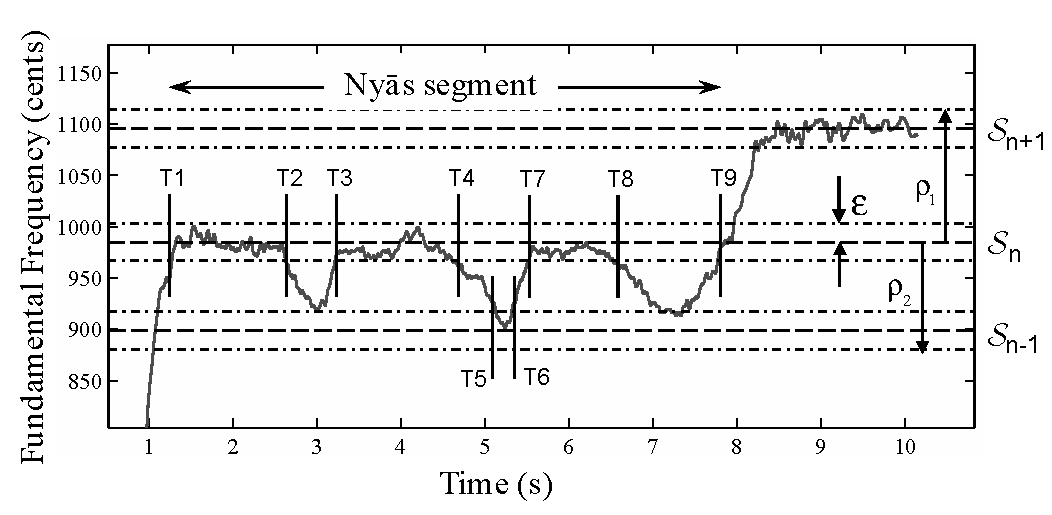
\includegraphics[width=\figSizeNinety]{ch05_preprocessing/figures/NyasSegmentationMethod_BW.pdf}
		\else
			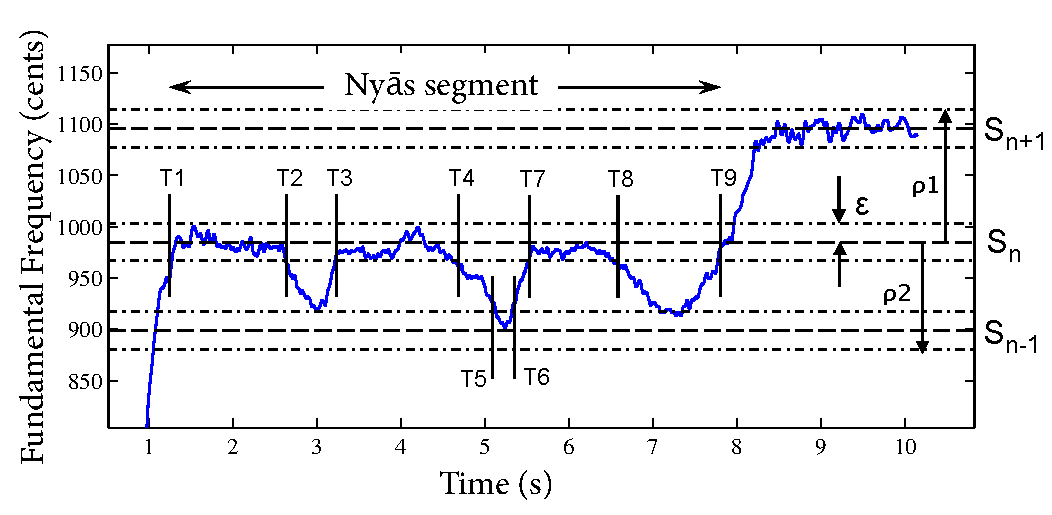
\includegraphics[width=\figSizeNinety]{ch05_preprocessing/figures/NyasSegmentationMethod.pdf}
		\fi
	\end{center}
	\caption[Illustration of the \gls{nyas} segmentation process]{Fragment of a pitch contour containing a \gls{nyas} segment ($\timeStamp_1-\timeStamp_9$), where $\timeStamp_i$s denote time stamps and $\freqSvara_n$s denote mean \gls{svara} frequencies. The pitch deviation within the \gls{nyas} segment ($\timeStamp_1-\timeStamp_9$) is almost 100\,Cents.}
	\label{fig:nyas_segmentation_illustration}
\end{figure}

We experiment with two different methods for segmenting melodies: \gls{pls}, a classical, generic approach used for the segmentation of time series data~\citep{keogh2004segmenting}, and our proposed method, which incorporates domain knowledge to facilitate the detection of \gls{nyas} boundaries. For \gls{pls} we use a bottom-up segmentation strategy as described by~\cite{keogh2004segmenting}. Bottom-up segmentation methods involve computation of residual error incrementally for each sample of time series. When the residual error satisfies a pre-defined criterion a new segment is created. Out of the two typical criteria used for segmentation, namely average and maximum error, we choose the latter because, ideally, a new segment should be created as soon as the melody progresses from one \gls{svara} to the other. In order to select the optimal value of the allowed maximum error, which we denote by $\maxErrorPLS$, we iterated over four different values and chose the one which resulted in the best performance. Specifically, for $\maxErrorPLS=\lbrace 10, 25, 50, 75\rbrace$, $\maxErrorPLS=75$\,cents yielded the best performance. We rejected $\maxErrorPLS\geq 100$\,cents in early experimentation stages because few \glspl{svara} of a \gls{raga} are separated by an interval of 100\,Cents and, therefore, the segmentation output was clearly unsatisfactory.

To make the segmentation process robust to pitch deviations, we propose a method based on empirically-derived thresholds. Unlike \gls{pls}, our proposed method computes a pitch histogram and uses that to estimate mean \gls{svara} frequencies before the computation of residual error. This allows us to compute the residual error with respect to the mean \gls{svara} frequency instead of computing it with respect to the previous segment boundary, as done in \gls{pls}. In this way our proposed method utilizes the fact that the time series being segmented is a pitch contour where the values of the time series hover around mean \gls{svara} frequencies. The mean \gls{svara} frequencies for an excerpt are estimated as the peaks of the histogram computed from the estimated pitch values. An octave folded pitch histogram is computed using a 10\,cent resolution and subsequently smoothened using a Gaussian window with a variance of 15\,cents. Only the peaks of the normalized pitch histogram which have at least one peak-to-valley ratio greater than 0.01 are considered as \gls{svara} locations. As peaks and valleys we simply take all local maximas and minimas over the whole histogram. In~\figref{fig:pitch_histogram_nyas_segmentation} we show an example of an octave folded normalized pitch histogram used for estimating mean \gls{svara} frequencies. The estimated mean \gls{svara} frequencies are indicated by circles. We also notice that the pitch values corresponding to a \gls{svara} span a frequency region and not a single value.


\begin{figure}
	\begin{center}
		\ifdefined\PRINTVER
			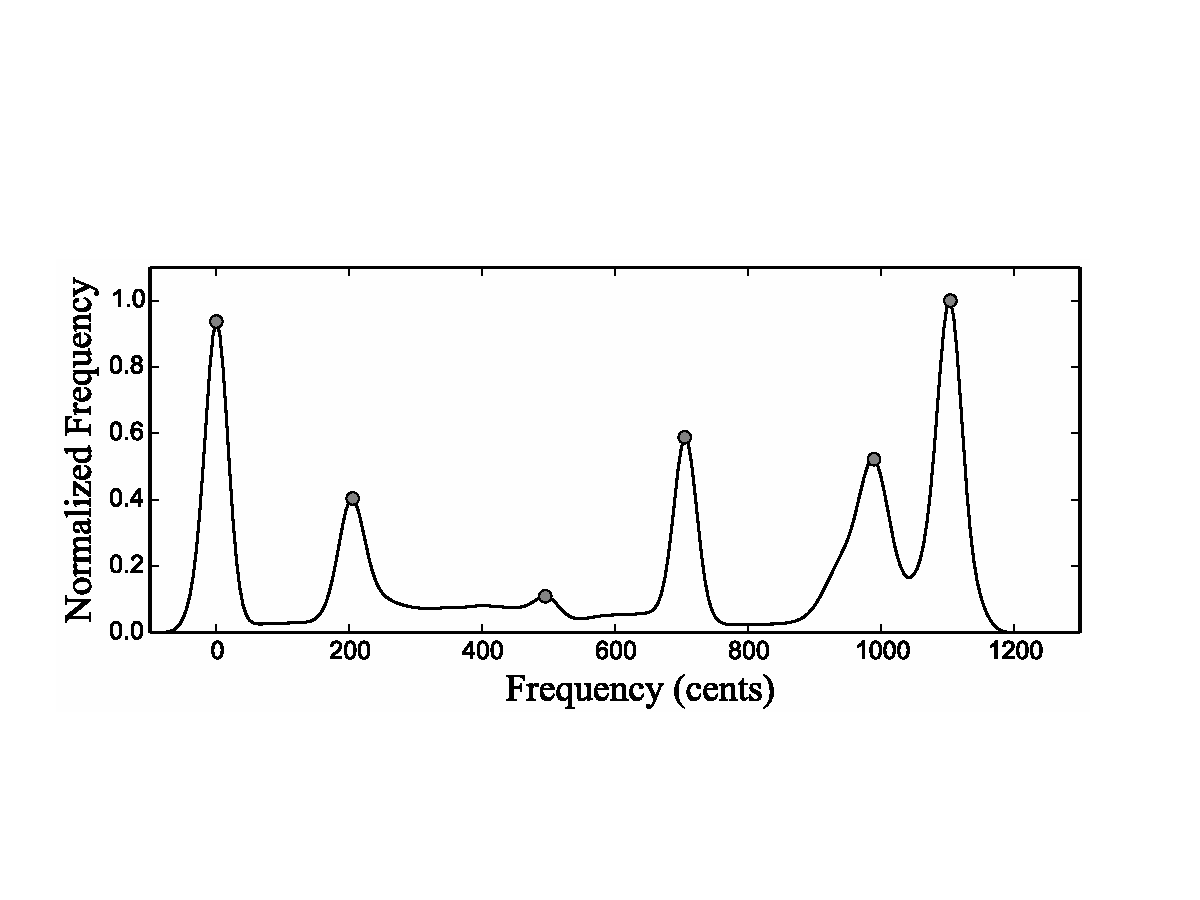
\includegraphics[width=\figSizeEighty]{ch05_preprocessing/figures/swarOnHistogramForNyasSegmentation_BW.pdf}
		\else
			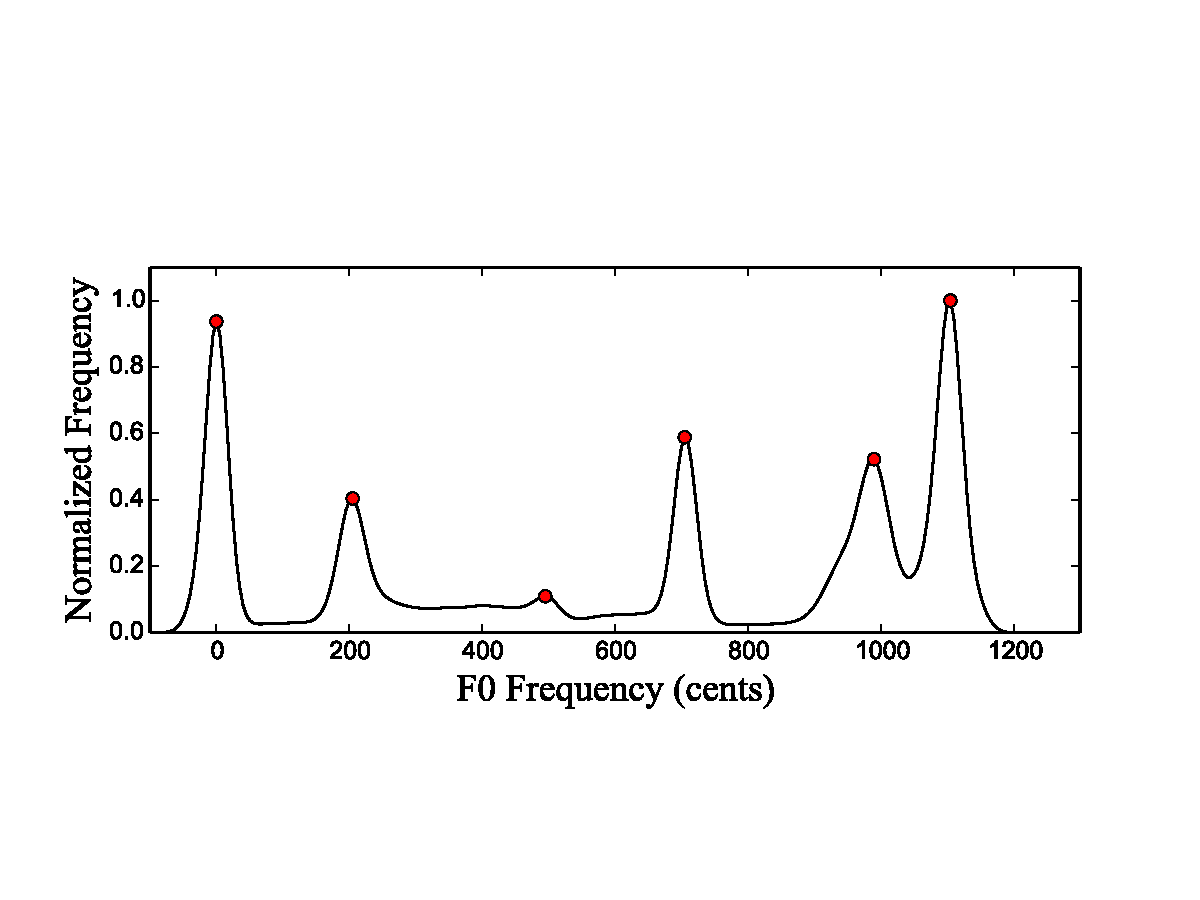
\includegraphics[width=\figSizeEighty]{ch05_preprocessing/figures/swarOnHistogramForNyasSegmentation.pdf}
		\fi
	\end{center}
	\caption[Example of a normalized octave folded pitch histogram]{Normalized octave folded pitch histogram used for estimating mean \gls{svara} frequencies. Estimated mean \gls{svara} frequencies are indicated by circles.}
	\label{fig:pitch_histogram_nyas_segmentation}
\end{figure}

After we estimate mean frequencies of all the \glspl{svara} in a piece, we proceed with their refinement. For the $n$-th \gls{svara} $\freqSvara_n$, we search for contiguous segments within a deviation of $\awdErrorNyas$ from $\freqSvara_n$, that is, $\vert \freqSvara_n-\pitchCents_i \vert < \awdErrorNyas$, for~$i\in[1,N]$, where $\pitchCents_i$ is the fundamental frequency value (in cents) of the $i$-th sample of a segment of length $N$. In Figure~\ref{fig:nyas_segmentation_illustration}, this corresponds to segments $[\timeStamp_1,\timeStamp_2]$, $[\timeStamp_3,\timeStamp_4]$, and $[\timeStamp_7,\timeStamp_8]$.

Next, we concatenate two segments $[\timeStamp_a,\timeStamp_b]$ and $[\timeStamp_e,\timeStamp_f]$ if two conditions are met:
\begin{enumerate}
	\item $\pitchCents_i-\freqSvara_n < \maxErrorNyas_1$ and $\freqSvara_n-\pitchCents_i < \maxErrorNyas_2$, for $i\in[\timeStamp_b,\timeStamp_e]$, where $\maxErrorNyas_1 = \freqSvara_{n+1}-\freqSvara_n + \awdErrorNyas$ and $\maxErrorNyas_2 = \freqSvara_n-\freqSvara_{n-1} + \awdErrorNyas$. 
	\item $\timeStamp_c-\timeStamp_d < \timeTshldNyas$, where $\timeTshldNyas$ is a temporal threshold and $[\timeStamp_c,\timeStamp_d]$ is a segment between $\timeStamp_b, \timeStamp_e$ such that $\vert \freqSvara_m-\pitchCents_i\vert <\awdErrorNyas$ for $i\in[\timeStamp_c,\timeStamp_d]$ for $m\in [{n-1}, {n+1}]$ and $m \neq n$.
\end{enumerate}

In simple terms, we concatenate two segments if the fundamental frequency values between them do not deviate a lot (less than $\maxErrorNyas_1$ and $\maxErrorNyas_2$) and the time duration of the melody in close vicinity (less than $\awdErrorNyas$) of neighboring \glspl{svara} is not too large (less than $\timeTshldNyas$). We repeat this process for all \gls{svara} locations. In our experiments, we use $\awdErrorNyas = 25$\,cents and $\timeTshldNyas=50$\,ms, which were empirically obtained. Notice that we can already derive a simple binary flatness measure $\binFlatNyas$ for $[\timeStamp_a, \timeStamp_b]$, $\binFlatNyas=1$ if $\vert \freqSvara_n-\pitchCents_i \vert< \awdErrorNyas$ for $i \in [\timeStamp_a, \timeStamp_b]$ for any $n$ and $\binFlatNyas=0$ otherwise. 

\subsubsection{Feature Extraction}
\label{sec:pro_processing_nyas_segmentation_feature_extraction}

We extract musically motivated melodic features for segment classification, which resulted out of discussions with musicians. For every segment obtained following the process mentioned above, three sets of melodic features are computed: local features~(\acrshort{nyas_local_feature}), which capture the pitch contour characteristics of the segment, contextual features~(\acrshort{nyas_context_feature}), which capture the melodic context of the segment, and a third set combining both of them~(\acrshort{nyas_local_feature}+\acrshort{nyas_context_feature}) in order to analyze if they complement each other. Initially, we considered 9 local features and 24 contextual features:

\begin{description}
	\item[Local Features:] segment length, mean and variance of the pitch values in a segment, mean and variance of the differences in adjacent peak locations of the pitch sequence in a segment, mean and variance of the peak amplitudes of the pitch sequence in a segment, temporal centroid of the pitch sequence in a segment normalized by its length, and the above-mentioned flatness measure $\binFlatNyas$ (we use the average segmentation error for the case of \gls{pls}).
	\item[Contextual Features:] segment length normalized by the length of the longest segment within the same breath phrase\footnote{Melody segment between consecutive breaths of a singer. We consider every unvoiced segment (i.e.,~a value of 0 in the pitch sequence) greater than 100\,ms as breath pause.}, segment length normalized by the length of the breath phrase, length normalized with the length of the previous segment, length normalized by the length of the following segment, duration between the ending of the segment and succeeding silence, duration between the starting of the segment and preceding silence, and all the local features of the adjacent segments.
\end{description}

However, after preliminary analysis, we reduced these features to 3 local features and 15 contextual features. As local features we selected length, variance, and flatness measure ($\binFlatNyas$). As contextual features we selected all of them except the local features of the posterior segment. This feature selection was done manually, performing different preliminary experiments with a subset of the data, using different combinations of features and selecting the ones that yielded the best accuracies.

\subsubsection{Classification and Segment Fusion}

Each segment obtained in~\secref{sec:nyas_svara_segmentation_method} is classified into \gls{nyas} or non-\gls{nyas} based on the extracted features described in~\secref{sec:pro_processing_nyas_segmentation_feature_extraction}. To demonstrate that the predictive power of the considered features is generic and independent of a particular classification scheme, we employ five different algorithms exploiting diverse classification strategies~\citep{Hastie09BOOK}: \gls{tree}, \gls{knn}, \gls{nb}, \gls{lr}, and \gls{svm} with a radial basis function kernel. We use the implementations available in scikit-learn~\citep{scikitlearn}, version 0.14.1. We use the default set of parameters with few exceptions in order to avoid over-fitting and to compensate for the uneven number of instances per class. Specifically, we set \texttt{min\_samples\_split=10} for \acrshort{tree}, \texttt{fit\_prior=False} for \gls{nb}, \texttt{n\_neighbors=5} for \gls{knn}, and for \gls{lr} and \gls{svm} \texttt{class\_weight=`auto'}.

For out-of-sample testing we implement a cross-fold validation procedure. We split the dataset into folds that contain an equal number of \gls{nyas} segments, the minimum number of \gls{nyas} segments in a musical excerpt. Furthermore, we make sure that no instance from the same artist and \gls{raga} is used for training and testing in the same fold.

After classification, boundaries of \gls{nyas} and non-\gls{nyas} segments are obtained by merging all the consecutive segments with the same segment label. During this step, the segments corresponding to the silence regions in the melody, which were removed during classification, are regarded as non-\gls{nyas} segments.

\subsection{Experimental Setup}
\label{sec:pre_processing_nyas_segmentation_experimental_setup}

\subsubsection{Music Collection and Annotations}

For evaluation of this task we use the \gls{nyas} dataset \acrshort{nds_cm} as described in~\secref{sec:corpus_nyas_dataset}. As explained, this dataset contains both commercially released polyphonic music recordings and in-house monophonic recordings. As melodic characteristics of a \gls{nyas} segment might depend on the artist and the chosen \gls{raga}, the dataset includes performances by 8 artists in 16 different \glspl{raga} to ensure diversity and representativeness.

\subsubsection{Evaluation Measures and Statistical Significance}

We evaluate two tasks, \gls{nyas} segment boundary annotation, and \gls{nyas} and non-\gls{nyas} segment label annotation. For the evaluation of \gls{nyas} boundary annotations we use hit rates as in a typical music structure boundary detection task~\citep{Ong05ICMC}. While calculating hit rate, segment boundaries are considered as correct if they fall within a certain threshold of a boundary in the ground-truth annotation. Using matched hits, we compute standard precision, recall, and F-score for every fold and average them over the whole dataset. The choice of a threshold however depends on the specific application. Due to the lack of scientific studies on the just noticeable differences of \gls{nyas} \gls{svara} boundaries, we computed results using an arbitrary selected threshold of 100\,ms. Label annotations are evaluated using standard pairwise frame clustering method as described in~\cite{levy2008structural}. Frames with same duration as threshold value for the boundary evaluation (i.e. 100~ms) are considered while computing precision, recall, and F-score. 

For assessing statistical significance we use the Mann-Whitney U test~\citep{mann1947test} with $\pVal<0.05$ and assuming an asymptotic normal distribution of the evaluation measures. To compensate for multiple comparisons we apply the Holm-Bonferroni method~\citep{holm1979simple}, a powerful method that also controls the so-called family-wise error rate. Thus, we end up using a much more stringent criterion than $\pVal<0.05$ for measuring statistical significance.

\subsubsection{Baselines}

Apart from reporting the accuracies for the proposed method and its variants, we compare against some baseline approaches. In particular, we consider \gls{dtw} together with a \gls{knn} classifier ($K=5$). For every segment, we compute its distance from all other segments and assign a label to it based on the labels of its $K$ nearest neighbors, using majority voting. As the proposed method also exploits contextual information, in order to make the comparison more meaningful, we consider the adjacent segments in the distance computation with linearly interpolated values in the region corresponding to the segment. For comparing with the variant of the proposed method that uses a combination of the local and contextual features, we consider adjacent segments together with the actual segment in the distance computation. As this approach does not consider any features, it will help us in estimating the benefits of extracting musically-relevant features from \gls{nyas} segments. 

In addition, to quantify the limitations of the adopted evaluation measures, we compute a few random baselines. The first one (\acrshort{nyas_randbase1}) is calculated by randomly planting boundaries (starting at 0\,s) according to the distribution of inter boundary intervals obtained using the ground-truth annotations. For each segment we assign the labels `\gls{nyas}' with a a priory probability (same for all excerpts) computed using ground truth annotations of the whole dataset. The second one (\acrshort{nyas_randbase2}) is calculated by planting boundaries (starting at 0\,s) at even intervals of 100\,ms and assigning class labels as in \acrshort{nyas_randbase1}. Finally, the third one (\acrshort{nyas_randbase3}) considers the exact ground-truth boundaries and assigns the class labels randomly as in \acrshort{nyas_randbase1} and \acrshort{nyas_randbase2}. Thus, with \acrshort{nyas_randbase3} we can directly assess the impact of the considered classification algorithms. We found that \acrshort{nyas_randbase2} achieves the best accuracy and therefore, for all the following comparisons we only consider \acrshort{nyas_randbase2}.

%\begin{table} 
%\centering
%\begin{tabular}{ c | c c c }
%\hline\hline
%  		&	\acrshort{nyas_randbase1}	&	\acrshort{nyas_randbase2}	&	\acrshort{nyas_randbase3}\\
%\hline
% 	\gls{nyas} Boundary		&  0.10 & 0.17 &1.0  \\ 
%%\hline 	
%	\gls{nyas} Region		& 0.56 & 0.69 & 0.64 \\
%\hline\hline
%\end{tabular}
%
%\caption{F-scores for \gls{nyas} boundary estimation and \gls{nyas} region
%estimation using random baseline methods. \XXX{J}{S}{Why not adding a row or column in the general results tables??}}
%	\label{tab:randombaseline}
%\end{table}

\subsection{Results and Discussion}
\label{sec:preprocessing_nyas_segmentation_results_and_discussion}

We evaluate two tasks, \gls{nyas} segment boundary annotation, and \gls{nyas} and non-\gls{nyas} segment label annotation. For both the tasks, we report results obtained using two different segmentation methods (\gls{pls} and the proposed segmentation method), five classifiers (\acrshort{tree}, \gls{knn}, \gls{nb}, \gls{lr}, \gls{svm}), and three set of features (local (\acrshort{nyas_local_feature}), contextual(\acrshort{nyas_context_feature}) and local together with contextual (\acrshort{nyas_local_feature}+\acrshort{nyas_context_feature})). In addition, we report results obtained using a baseline method (\acrshort{dtw}) and a random baseline (\acrshort{nyas_randbase2}).

In Table~\ref{tab:nyas_segmentation_boundary_accuracy}, we show the results of \gls{nyas} boundary annotations. First, we see that every variant performs significantly better than the best random baseline. \acrshort{nyas_randbase2} yields an F-score of 0.184 while the worst variant tested reaches 0.248. Next, we see that the proposed method achieves a notably higher accuracy compared to the \acrshort{dtw} baseline. Such difference is found to be statistically significant, with the only exception of the \acrshort{nb} classifier. For a given feature set, the performance differences across classifiers are not statistically significant. The only exceptions are \acrshort{tree} and \acrshort{nb}, which yield relatively poor and inconsistent performances over different feature sets. Therefore, we opted to not consider these two classifiers in the following comparisons. Amongst the feature sets, the performance differences are not statistically significant between \gls{pls} variants (Table~\ref{tab:nyas_segmentation_boundary_accuracy}, top rows), whereas for the case of the proposed segmentation method (Table~\ref{tab:nyas_segmentation_boundary_accuracy}, bottom rows), we find that the local features perform significantly better than the contextual features and their combination does not yield consistent improvements. Finally, we see that the best results are obtained using the proposed segmentation method together with the local features, with a statistically significant difference to its competitors. Furthermore, the worst accuracy obtained using the proposed segmentation method is notably higher than the best accuracy using \gls{pls} method, again with a statistically significant difference.

\begin{table} 
\renewcommand{\arraystretch}{1.25}
\setlength{\tabcolsep}{6pt}
	\begin{centering}
	\begin{tabular}{ c : c : c : c c c c c c }
\tabletop
		& Feat.		&	\gls{dtw} & \acrshort{tree}	 &	\gls{knn} 	&	\gls{nb}		& \gls{lr} 	&	\gls{svm}\\
\tablemid
		\multirow{3}{*}{A} & 	\acrshort{nyas_local_feature}		&  0.356 & 0.407 & 0.447 & 0.248 & 0.449 & 0.453\\ 
		%\hline 	
		&	\acrshort{nyas_context_feature}		& 0.284 & 0.394 & 0.387 & 0.383 & 0.389 & 0.406 \\
		%\hline	
		&	\acrshort{nyas_local_feature}+\acrshort{nyas_context_feature}		& 0.289 & 0.414 & 0.426 & 0.409 &0.432 & 0.437 \\
\tablemid
		\multirow{3}{*}{B} &	\acrshort{nyas_local_feature}		& \textbf{0.524} & 0.672 & \textbf{0.719} & 0.491 & \textbf{0.736} & \textbf{0.749}\\ 
		%\hline 	
		&	\acrshort{nyas_context_feature}		& 0.436 & 0.629 & 0.615 & \textbf{0.641} & 0.621 & 0.673 \\
		%\hline	
		&	\acrshort{nyas_local_feature}+\acrshort{nyas_context_feature}		& 0.446 & \textbf{0.682} & 0.708 & 0.591 & 0.725 & 0.735\\  		
\tablebot		
	\end{tabular}	
	\caption[F-scores for the \gls{nyas} boundary detection task]{F-scores for \gls{nyas} boundary detection using \gls{pls} method (A) and the proposed segmentation method (B). Results are shown for different classifiers (\acrshort{tree}, \gls{knn}, \gls{nb}, \gls{lr}, \gls{svm}) and local (\acrshort{nyas_local_feature}), contextual (\acrshort{nyas_context_feature}) and local together with contextual (\acrshort{nyas_local_feature}+\acrshort{nyas_context_feature}) features. \gls{dtw} is the baseline method used for comparison. F-score for the random baseline obtained using \acrshort{nyas_randbase2} is 0.184.}
	\label{tab:nyas_segmentation_boundary_accuracy}
	\par	\end{centering}
\end{table}


In~\tabref{tab:nyas_segmentation_label_accuracies}, we show the results for \gls{nyas} and non-\gls{nyas} label annotations. We can draw similar conclusions as with Table~\ref{tab:nyas_segmentation_label_accuracies}: (1) all the method variants perform significantly better than the random baselines, (2) all the proposed method variants yield significant accuracy increments over the \GLS{dtw} baseline, and (3) no statistically significant differences between classifiers (with the aforementioned exceptions). In the label annotations, unlike the boundary annotations, we find that though the local features perform better than the contextual features, the differences are not statistically significant for all the proposed method variants. Furthermore, we also see that the proposed segmentation method consistently performs better than \gls{pls}. However, the differences are not always statistically significant.

In addition, we also investigate per-class accuracies for the label annotations. We find that the performance for the \gls{nyas} segments is considerably better than the non-\gls{nyas} segments. This could be attributed to the fact that even though the segment classification accuracy is balanced across classes, the differences in segment length of \gls{nyas} and non-\gls{nyas} segments (\gls{nyas} segments being considerably longer than non-\gls{nyas} segments) can result in more number of matched pairs for \gls{nyas} segments.

\begin{table} 
\renewcommand{\arraystretch}{1.25}
\setlength{\tabcolsep}{6pt}
\begin{centering}	
	\begin{tabular}{ c : c : c : c  c  c  c  c  c }
\tabletop
		& Feat.	&	\acrshort{dtw} & \acrshort{tree}	 &	\acrshort{knn} 	&	\acrshort{nb}		& \acrshort{lr} 	&	\acrshort{svm}	\\
\tablemid		
		\multirow{3}{*}{A} &   \acrshort{nyas_local_feature}		& \textbf{0.553} & 0.685 & 0.723 & 0.621 & 0.727 & 0.722	\\
		%\hline         
		&	\acrshort{nyas_context_feature}   		& 0.251 & 0.639 & 0.631  & 0.690 & 0.688 & 0.674	\\
		%\hline 
		& 	\acrshort{nyas_local_feature}+\acrshort{nyas_context_feature}		& 0.389 & 0.694 & 0.693 & 0.708 & 0.722 & 0.706	\\	
		\hline
		\multirow{3}{*}{B} & 	\acrshort{nyas_local_feature}		& 0.546 & \textbf{0.708} & \textbf{0.754} & 0.714 & \textbf{0.749} & \textbf{0.758} \\
		%\hdashline 	
		& 	\acrshort{nyas_context_feature}		&0.281 & 0.671 & 0.611 & 0.697 & 0.689 & 0.697\\
		%\hline	
		& 	\acrshort{nyas_local_feature}+\acrshort{nyas_context_feature}		& 0.332 & 0.672 & 0.710 & \textbf{0.730} & 0.743 & 0.731\\
\tablebot
	\end{tabular}
	\caption[F-scores for the \gls{nyas} and non-\gls{nyas} label annotation task]{F-scores for \gls{nyas} and non-\gls{nyas} label annotation task using \gls{pls} method (A) and the proposed segmentation method (B). Results are shown for different classifiers (\acrshort{tree}, \acrshort{knn}, \acrshort{nb}, \acrshort{lr}, \acrshort{svm}) and local (\acrshort{nyas_local_feature}), contextual (\acrshort{nyas_context_feature}) and local together with contextual (\acrshort{nyas_local_feature}+\acrshort{nyas_context_feature}) features. \acrshort{dtw} is the baseline method used for comparison. The best random baseline F-score is 0.153 obtained using \acrshort{nyas_randbase2}. } 
	\label{tab:nyas_segmentation_label_accuracies}
\par \end{centering}
\end{table}


In general, we see that the proposed segmentation method improves the performance over \gls{pls} method in both the tasks, wherein the differences are statistically significant in the former case. Furthermore, the local feature set, when combined with the proposed segmentation method, yields the best accuracies. We also find that the contextual features do not complement the local features to further improve the performance. However, interestingly, they perform reasonably good considering that they only use contextual information.


\subsection{Summary}
\label{ConclusionAndFutureWork}

We described a method for detecting \gls{nyas} segments in melodies of Hindustani music. We divided the task into two broad steps: melody segmentation and segment classification. For melody segmentation we proposed a method which incorporates domain knowledge to facilitate \gls{nyas} boundary annotations. We evaluated three feature sets: local, contextual and the combination of both. We showed that the performance of the proposed method is significantly better compared to a baseline method using standard \gls{dtw} based distance and a \gls{knn} classifier. Furthermore, we showed that the proposed segmentation method outperforms a standard approach based on \gls{pls}. A feature set that includes only the local features was found to perform best. However, we showed that using just the contextual information we could also achieve a reasonable accuracy. This indicates that \gls{nyas} segments have a defined melodic context which can be learned automatically. 


\section{Tani Segmentation}
\label{sec:pre_processing_tani_segmentation}

A concert of Carnatic music typically contains a solo percussion section towards the end of the concert, referred to as \gls{tani} avartanam or \gls{tani} in short. The duration of this section typically varies from 2 to 25\,min depending on the artist and the context. The main percussion instrument in Carnatic music is \gls{mridangam}, which becomes the lead instrument during this section. Along with the \gls{mridangam} there are other percussion instruments often played in \gls{tani} section such as \gls{kanjira} and \gls{ghatam}. Though \gls{mridangam} is a percussion instrument and is basically a kind of a barrel drum, its sound has tonal characteristics. Like the other accompanying instruments in Carnatic music such as \gls{tanpura} and violin, \gls{mridangam} is also tuned at the tonic of the lead artist. Due to the tonal acoustical characteristics of \gls{mridangam} sound, and because of the long duration of \gls{tani} sections, the pitch estimation algorithm detects and tracks pitch contours during the \gls{tani} sections, instead of detecting these sections as non-voiced segments. Notice that the \gls{mridangam} strokes during short (lasting over roughly 1-20 seconds) unvoiced segments such as breath-pauses are correctly detected as non-voiced by the predominant pitch estimation algorithm. This is due to the fact that during such sections the predominant pitch corresponds to the voice, which has significantly higher energy compared to the background percussion signal. 


\begin{figure}
	\begin{center}
		\ifdefined\PRINTVER
			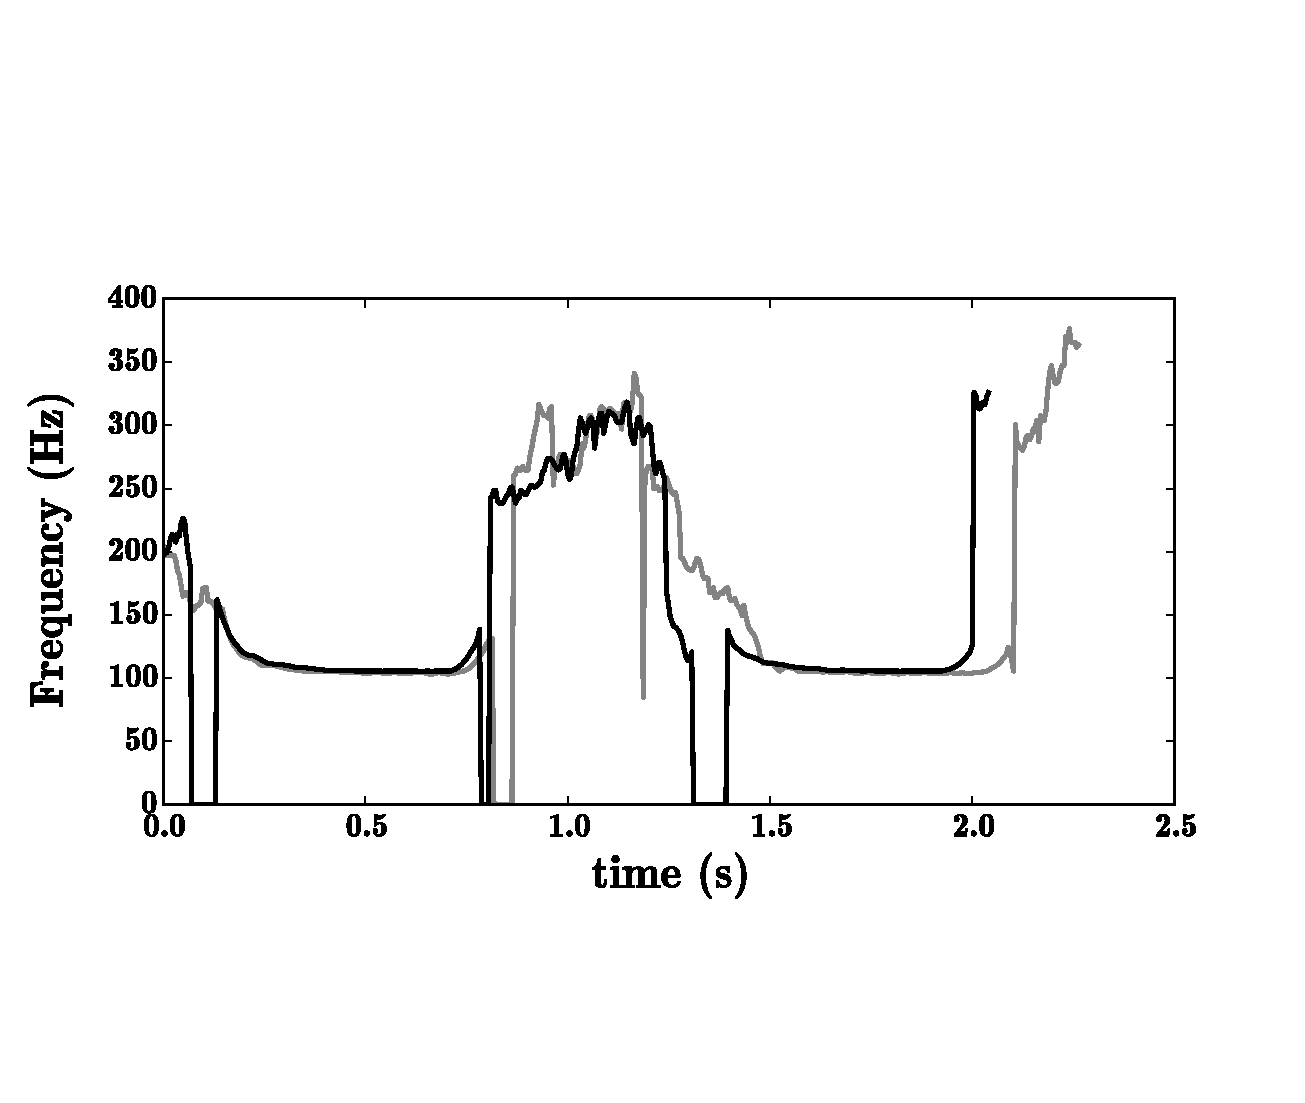
\includegraphics[width=\figSizeSeventy]{ch05_preprocessing/figures/taniPatterns_BW.pdf}
		\else
			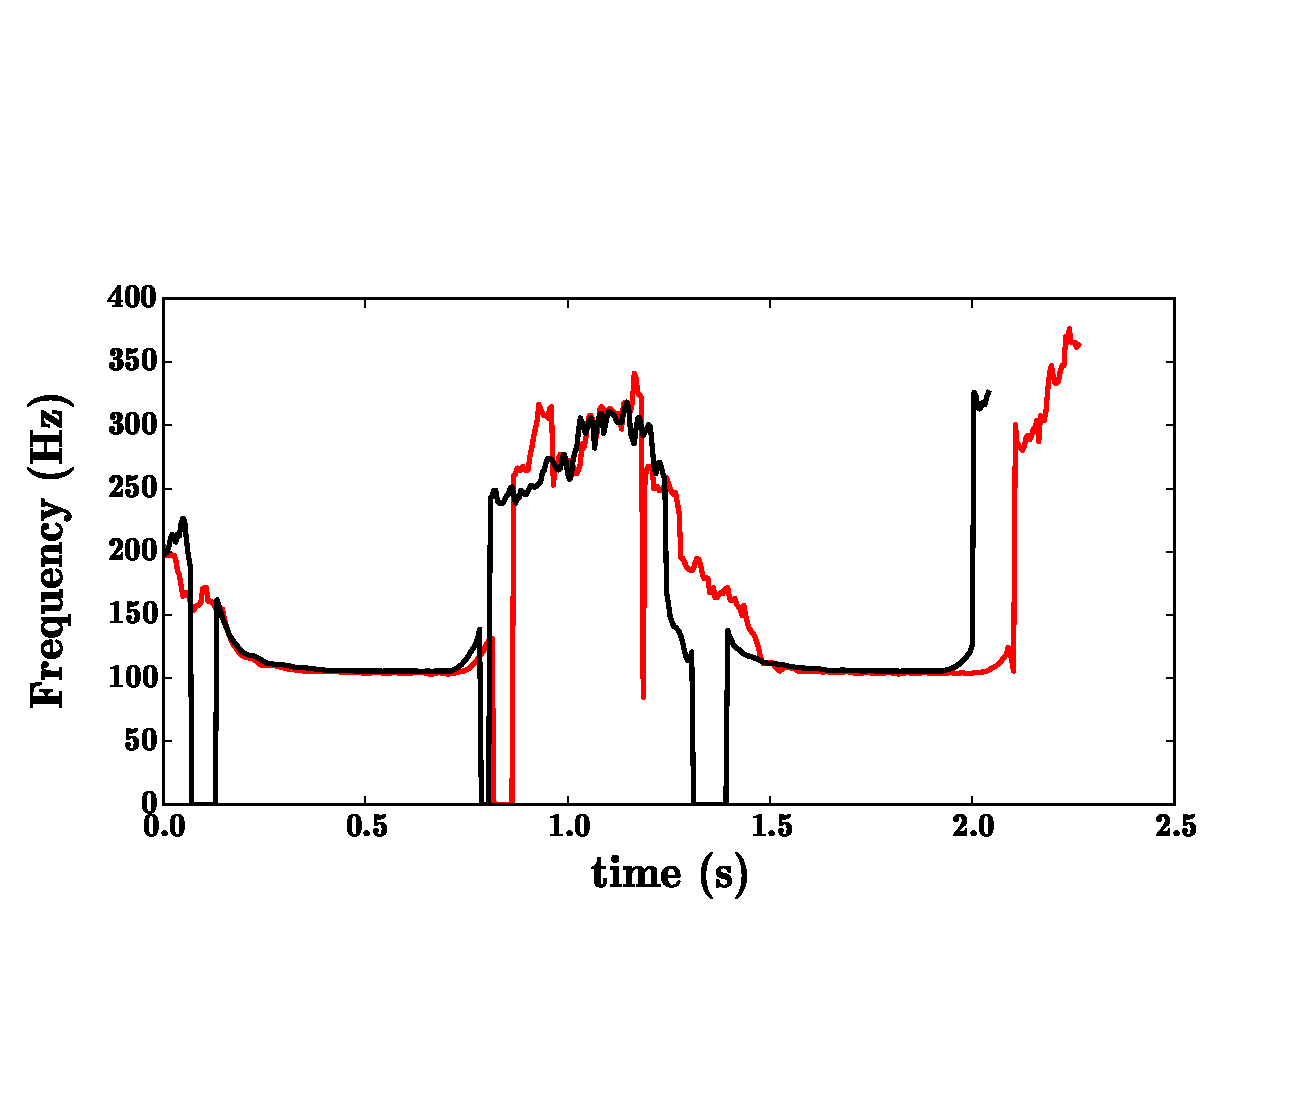
\includegraphics[width=\figSizeSeventy]{ch05_preprocessing/figures/taniPatterns.pdf}
		\fi
	\end{center}
	\caption[Melodic patterns corresponding to the \gls{mridangam} strokes]{Pitch contours of a pair of highly similar melodic patterns corresponding to the \gls{mridangam} strokes in a \gls{tani} section.}
	\label{fig:pitch_pattern_tani}
\end{figure}

Detecting pitch corresponding to the \gls{mridangam} strokes as predominant pitch in the audio poses several challenges in melodic analyses, specifically in the discovery of melodic patterns. Percussion patterns and rhythm cycles contain recurring strokes (or patterns), and therefore, pitch fragments from the \gls{tani} section are frequently discovered as highly similar patterns. An example of a discovered pair of pitch patterns that correspond to \gls{mridangam} strokes is shown in~\figref{fig:pitch_pattern_tani}. We see that the patterns are close to exact repetitions. Since we aim to discover patterns in melodies of \gls{iam} (\chapref{chap:melodic_pattern_processing}), patterns discovered from the \gls{tani} sections are undesired. There can be two approaches to avoid such unwanted patterns in the final output: 1) post-process the discovered pitch patterns and detect if they belong correspond to \gls{mridangam} strokes, 2) discard pitch contours corresponding to the \gls{tani} section in the pre-processing step. We follow the second approach and discard segments of the pitch contours that correspond to the \gls{tani} sections from the input given to the pattern discovery method. Discarding such segments upfront has several advantages. First, detection of the \gls{tani} sections in audio recording appears to be an easier task compared to characterizing pitch contours as belonging to the melody or \gls{mridangam} strokes. This is mainly because of the considerable amount of timbral differences across the sections where melody is present and where it is not. In addition, such computational tasks of classifying an audio segment based on its timbral characteristics is well studied in \gls{mir}~\citep{herrera2003automatic}. In~\figref{fig:spectrogram_of_tani_segment}, we show the spectrogram of a voice section and a \gls{tani} section. We see that the timbral characteristics between the two types of sections are considerably different. Another benefit of discarding the \gls{tani} sections upfront is that it reduces the computational complexity of the pattern discovery task (\gls{tani} sections may last up to 2-25\,minutes). %We therefore detect \gls{tani} sections directly in the audio recordings and discard the pitch segments corresponding to these sections in the pre-processing step.

\begin{figure}
	\begin{center}
		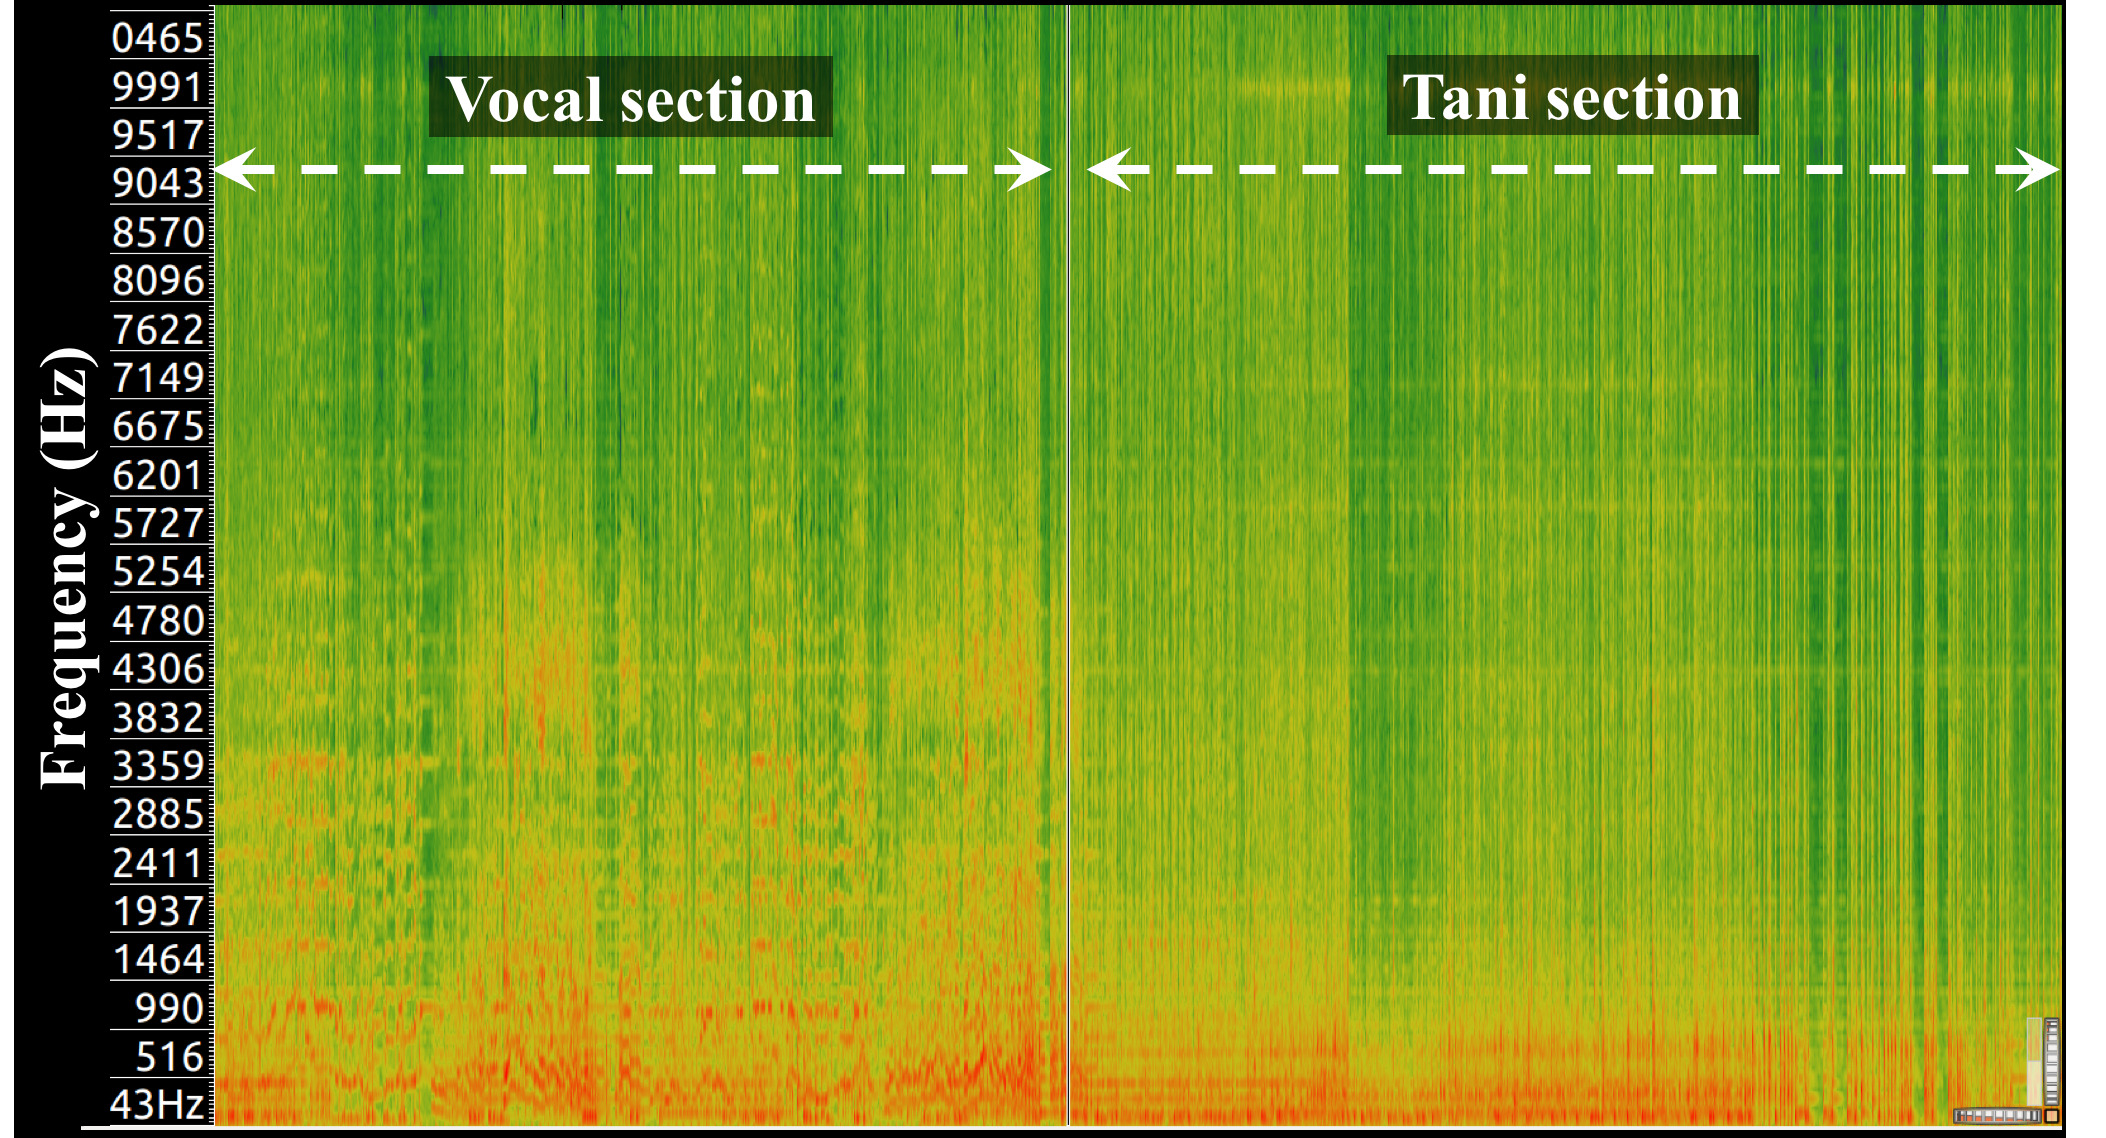
\includegraphics[width=\figSizeEighty]{ch05_preprocessing/figures/spectrogramTani.png}
	\end{center}
	\caption[Illustration of the spectrogram a vocal and a \gls{tani} section]{The spectrogram of a voice (with percussion) and a \gls{tani} section in an audio recording of Carnatic music. The excerpt spans 3\,minutes of audio.}
	\label{fig:spectrogram_of_tani_segment}
\end{figure}

We detect \gls{tani} sections in audio recordings using a classification-based approach. To feed the classifiers we extract 13~\acrshort{mfcc} coefficients, spectral centroid, spectral flatness and pitch salience from the audio signal using Essentia~\citep{essentia} library. We iterate over 23, 46 and 92\,ms frame sizes and chose the one that results in the best classification accuracy. We set the hop size as half the frame size and all other parameters to their default values. Next, we compute the means and the variances of these features over 2\,s non-overlapping segments (sometimes referred to as texture window). For training, we use a labeled audio music dataset containing 1.5~hours of mixed voice and violin recordings and 1.5~hours of solo percussion recordings. To assess the performance of the extracted features, we perform a 10-fold cross-validation procedure and repeat the experiment 10 times. We experiment with five different algorithms exploiting diverse classification strategies~\citep{Hastie09BOOK}: decision trees (\acrshort{tree}), \gls{knn}, \gls{nb}, \gls{lr}, and \gls{svm} with a radial basis function kernel. We use the implementations of the classifiers as available in scikit-learn version~0.14.1~\citep{scikitlearn}. We used the default set of parameters with few exceptions to avoid over-fitting and to compensate for the uneven number of instances per class. We set \texttt{min\_} \texttt{samples\_split=10} for \acrshort{tree}, \texttt{fit\_prior=False} for \gls{nb}, \texttt{n\_neighbors=5} for \gls{knn}, and for \gls{lr} and \gls{svm} \texttt{class\_weight=`auto'}. 

The combination of the frame size of 46\,ms and the \gls{svm} classifier yielded the best performance (96\% accuracy), with no statistically significant difference to the performance with the \acrshort{tree} (95.5\%) and the \gls{knn} (95\%), for the same frame size. We finally chose \gls{knn} because of its low complexity. Detection accuracy of the \gls{tani} sections can be improved further by a simple post-processing step. Since \gls{tani} is a single continuous section in an audio recording, class labels of the texture windows predicted by the classifier can be median filtered to remove the spurious labels lasting over a few frames. This ensures continuity of the class labels across texture windows and avoids short non-voiced regions during the vocal sections being classified as \gls{tani} segments. 

\section{Summary}
\label{sec:preprocessing_summary}

%\XXX{S}{J}{I am finding it difficult to describe the contents of this chapter in a single concept (descriptors or representations). Strictly speaking, referring to nyas segmentation as melodic descriptors is misleading. Its already a higher level analysis. If you have any suggestion to change the way I introduce this chapter or to group these 4 different sections please let me know.}

In this chapter, we described methods to obtain relevant melodic descriptors and melody representations from audio recordings. We presented algorithms used to extract and post-process the predominant pitch from these recordings. To match the tonal context of melodies across performances, the predominant pitch is normalized by the tonic used in the recordings. We presented an exhaustive evaluation of a number of tonic identification approaches, wherein we analyzed and compared their performance on different music material such as Hindustani and Carnatic music, male and female singers, and for instrumental and vocal music. We showed that our multipitch approach consistently outperformed all the other methods. Subsequently, we described our \gls{nyas}-based approach for segmenting melodies in Hindustani music. We saw that a knowledge driven segmentation approach performs better than a generic method for segmenting time-series data. In addition, we showed that our classification-based approach that uses abstracted melodic features performs better than a string matching based method for labeling \gls{nyas} segments. Furthermore, we demonstrated the utility of the context-based melodic features for \gls{nyas} detection task. At the end of the chapter, we explained our methodology for identifying \gls{tani} sections in recordings of Carnatic music. We showed that a classification-based approach that uses timbral features can successfully identify \gls{tani} sections with accuracy.

%\COMMENT{Somehow I am not able to write nicely a summary of this chapter. Please let me know if you clearly see what's missing.}
%

